\documentclass[tid,table]{texufpel} %use tid para doutorado e ti para mestrado



\usepackage{enumerate}
\usepackage[utf8]{inputenc} % acentuacao
\usepackage{graphicx} % para inserir figuras
\usepackage{url}

\hypersetup{
    hidelinks, % Remove coloração e caixas
    unicode=true,   %Permite acentuação no bookmark
    linktoc=all %Habilita link no nome e página do sumário
}

\usepackage{xcolor}
\usepackage{tabularx}
\usepackage{tablefootnote}

\usepackage{pdflscape}
\usepackage{afterpage}
\usepackage{capt-of}% or use the larger `caption` package

\usepackage[color=green!40]{todonotes}
\newcommand {\AY} {\todo[inline, color=green]} %comentarios Adenauer
\newcommand {\AP} {\todo[inline, color=yellow]} %Comentarios Ana

\unidade{Centro de Desenvolvimento Tecnológico}
\programa{Programa de Pós-Graduação em Computação}
\curso{Ciência da Computação}


\title{Avaliação de Estratégias de Segurança Adaptativa para a Internet das Coisas}


% VER ORIENTACAO DO LUCAS

\author{Almeida}{Ricardo Borges}
\advisor[Prof\textsuperscript{a}.~Dr\textsuperscript{a}.]{Pernas}{Ana Marilza}
\coadvisor[Prof.~Dr.]{Yamin}{Adenauer Corrêa}
\coadvisor[Sr.]{Donato}{Lucas Medeiros}

\keyword{Internet das Coisas}
\keyword{Segurança Adaptativa}
\keyword{Ciência de Contexto}

%Palavras-chave em EN_US
\keywordeng{Internet of Things}
\keywordeng{Adaptive Security}
\keywordeng{Context Awareness}
%\keywordeng{keyword-four}

\begin{document}

%\renewcommand{\advisorname}{Orientadora}           %descomente caso tenhas orientadora
\renewcommand{\coadvisorname}{Coorientadora}      %descomente caso tenhas coorientadora

\maketitle 

\sloppy

%\fichacatalografica


\begin{abstract}
Uma materialização da Computação Ubíqua que vem ganhando destaque é a Internet das Coisas (IoT), a qual consiste de um ecossistema que combina redes de sensores com e sem fio, computação em nuvem, dados analíticos, tecnologias interativas, bem como dispositivos inteligentes. A IoT atualmente inclui uma gama diversificada de dispositivos, serviços e redes para se tornar uma internet de qualquer coisa, em qualquer lugar, de qualquer forma e a qualquer momento. Com isso, os desafios de segurança e privacidade se potencializaram enquanto características necessárias e viabilizadoras para IoT. Promover a segurança com mecanismos pré-definidos e estáticos sobre este ambiente dinâmico e heterogêneo não se mostra mais uma abordagem oportuna. Por isso, são necessárias soluções para segurança auto-adaptativa. Tendo isto em vista, os objetivos deste trabalho consistem em: (i) sistematizar e apresentar os conceitos sobre segurança adaptativa para IoT, incluindo a sua relação com os estudos em ciência de contexto; (ii) realizar um mapeamento sistemático da literatura buscando identificar o estado da arte em segurança adaptativa para IoT; e (iii) desenvolver uma análise crítica sobre os trabalhos identificados em um esforço para elencar as lacunas existentes nesta área.
\end{abstract}


\begin{englishabstract}%
  {Assessment of Adaptive Security Strategies for the Internet of Things}
One of Ubiquitous Computing most prominent materializations is the Internet of Things (IoT), which consists of an ecosystem that combines wireless and wired sensor networks, cloud computing, analytical data, interactive technologies as well as intelligent devices. IoT currently includes a diverse range of devices, services and networks to become an internet of anything, anywhere, any way and anytime. As a result, the security and privacy challenges have become potentialized as a necessary and viable feature for IoT. Promoting security over this dynamic and heterogeneous environment with pre-defined and static security mechanisms is a challenging task. Therefore, solutions for self-adaptive security are required. The objectives of this work are: (i) systematize and present the concepts of adaptive security for IoT, including its relation with studies in context awareness; (ii) perform a systematic mapping of the literature striving to identify the state of the art in adaptive security for IoT; and (iii) develop a critical analysis of the work identified in an effort to fill the gaps in this area.
\end{englishabstract}

%Lista de Figuras
\listoffigures

%Lista de Tabelas
\listoftables

%lista de abreviaturas e siglas
\begin{listofabbrv}{SPMDRT}
	\item[ARM] \textit{Adaptive Risk Management}
        \item[CERP-IoT] \textit{Cluster of European Research Projects on the Internet of Thing}
	\item[HP] \textit{Hewlett-Packard}
        \item[IBM] \textit{International Business Machines}
        \item[IDS] \textit{Intrusion Detection System}
	\item[IoT] Internet das Coisas
        \item[IP] \textit{Internet Protocol}
        \item[ISMS] \textit{Information Security Management System}
        \item[ISRM] \textit{Information Security Risk Management}
        \item[MAPE-K] \textit{Monitor-Analyze-Plan-Execute plus Knowledge}
        \item[OWASP] \textit{Open Web Application Security Project}
        \item[PDCA] \textit{Plan-Do-Check-Act}
        \item[QoS] \textit{Quality of Service}
        \item[RBAC] \textit{Role-Based Access Control}
        \item[RFID] \textit{Radio Frequency Identification}
	\item[UbiComp] \textit{Ubiquitous Computing}
        \item[WAF] \textit{Web Application Firewall} 
\end{listofabbrv}

%Sumario
\tableofcontents

%\listoftodos
%%%%%%%%%%%%%%%%%%%%%%%%%%%%%%%%%%%%%%%%%%%%%%%%%%%%%%%%%%%%%%%%%%%%%%%
\chapter{Introdução}

Com os avanços significativos das diversas tecnologias que permeiam as redes de computadores, especialmente aqueles proporcionados pelas pesquisas em torno da Computação Ubíqua (UbiComp), houve uma transformação na forma em que se busca, acessa e compartilha as informações, tornando o ambiente mais interativo, adaptável e informativo \cite{tweneboah17}. Uma materialização da UbiComp que vem ganhando destaque é a Internet das Coisas, do inglês \textit{Internet of Things} (IoT), a qual consiste de um ecossistema que combina redes de sensores sem fio, computação em nuvem, dados analíticos, tecnologias interativas, bem como dispositivos inteligentes. Seu objetivo é prover soluções nas quais os objetos são primordialmente concebidos de forma a usufruir da conectividade da rede para coleta e troca de dados por meio de um identificador que busca melhorar as interações objeto-a-objeto. 

O termo IoT foi cunhado em 1999 no \textit{Massachusetts Institute of Technology} pelo analista britânico Kevin Ashton, sendo inicialmente proposto para conectar coisas específicas através da Internet usando dispositivos, como \textit{Radio Frequency Identification} (RFID), para realizar a identificação e gerenciamento inteligente de produtos \cite{ashton09}. Desde então, esta visão foi expandida contemplando características da UbiComp concebidas por Mark Weiser (1991)\nocite{weiser91}, incluindo uma gama diversificada de dispositivos, serviços e redes para se tornar uma internet de qualquer coisa, em qualquer lugar, de qualquer forma e a qualquer momento. 

Esta proliferação de dispositivos conectados criou uma nova lacuna na segurança tradicional. O crescimento da IoT impulsionado pelas demandas do mercado inspirou novas tecnologias e protocolos, no entanto, os fabricantes tem concebido produtos mais rapidamente do que a segurança pode ser inserida desde o início deste processo \cite{sans17}. Com isso, os desafios de segurança e privacidade se potencializaram enquanto características necessárias e viabilizadoras para IoT, ou seja, o desenvolvimento da IoT é fortemente dependente do atendimento das preocupações de segurança \cite{sicari15}.


As ameaças e vulnerabilidades associadas à IoT são proporcionais as superfícies de ataque \cite{sans17}. Esses dispositivos sofrem ataques contra interfaces físicas, comunicação sem fio, protocolos de roteamento e ataques tradicionais vistos em redes \textit{Internet Protocol} (IP). Estudos realizados pela \textit{Open Web Application Security Project } (OWASP) e pela \textit{Hewlett-Packard} (HP) detalham uma série de vulnerabilidades que a IoT precisa abordar. O relatório destaca que 60\% das interfaces web disponíveis em dispositivos da IoT são propensas a ataques; 90\% desses dispositivos coletam pelo menos uma informação pessoal; 70\% se comunicam através de canais não criptografados; e 70\% são suscetíveis a ataques de enumeração de contas \cite{hpiot15, owaspiot18}. Estas são algumas preocupações graves, especialmente para os serviços de saúde apoiados na IoT, onde o tipo de informação tratada é principalmente pessoal.

As principais tecnologias promotoras da IoT são consideradas objetos sensoriais que possuem limitações de processamento, memória e armazenamento, além de preocupações com o consumo de energia. Desta forma,, as soluções de segurança atuais, como firewall, \textit{Intrusion Detection System} (IDS), \textit{Web Application Firewall} (WAF), até mesmo pequenos programas de antivírus, não são viáveis para essa rede de sensores de recursos reduzidos. Além disso, um incidente de segurança geralmente consiste em múltiplos vetores de ataque, com diferentes alvos visando explorar qualquer vulnerabilidade existente. Logo, essas soluções que se limitam a analisar informações contextuais específicas, por exemplo, informações do tráfego da rede ou de arquivos locais, não fornecem um contexto holístico para análise de risco, podendo produzir falsos positivos e negativos, resultando em decisões inadequadas de mitigação \cite{aman15}. 

% [ric] mesma duvida anterior
%\AY{Promover a segurança sobre este ambiente cujas dinamicidade e heterogeneidade são crescentes com mecanismos de segurança pré-definidos e estáticos não se mostra mais uma abordagem oportuna.}
Promover a segurança com mecanismos pré-definidos e estáticos sobre este ambiente dinâmico e heterogêneo não se mostra mais uma abordagem oportuna. Por isso, são necessárias soluções para segurança auto-adaptativa \cite{evesti13a}. Esses sistemas auto-adaptativos podem ser estáticos ou dinâmicos em termos de quando a adaptação ocorre. Neste segundo caso, o processo é apoiado por um clico de \textit{feedback} que permite que os sistemas tomem suas próprias decisões de adaptação sem intervenção humana \cite{lamprecht12}. Desta forma, uma vez que este texto tem interesse particular na adaptação dinâmica, em tempo de execução, o termo adaptação será usado como sinônimo para auto-adaptação.

A segurança adaptativa, visa selecionar automaticamente mecanismos de segurança e seus parâmetros em tempo de execução para preservar o nível de segurança requerido em um ambiente em mudança \cite{evesti13a}. Isso é buscado  por meio do monitorando de atributos e ações que afetam a segurança atual e a desejada. Quando uma diferença entre a segurança atual e a necessária é identificada, os mecanismos de segurança são modificados. Nesta pesquisa, o foco está na adaptação baseada em arquitetura, onde o sistema considera o próprio modelo em conjunto com o seu ambiente, e se adapta quando necessário de acordo com alguns objetivos de adaptação.

A adaptação, ou comportamento autonômico é considerado um desafio importante da IoT \cite{aman16, alaba17, gartnerttrends17}. Esse desafio está relacionado à capacidade de dispositivos e aplicações adaptarem seu comportamento como resposta às mudanças em seu ambiente de operação. Desta forma, a segurança adaptativa decorre do fato que os sistemas enfrentam ambientes e situações distintas durante sua operação que requerem diferentes objetivos de segurança. Ou seja, em algumas situações, a integridade é um objetivo de segurança essencial, mas em outras a autenticação tem maior prioridade. Adicionalmente, a criticidade da informação varia entre as situações, em alguns casos a aplicação pode operar com dados de acesso público, em outros, com dados sensíveis como informações sobre a saúde de pacientes. Portanto, o nível de segurança requerido varia de uma situação para outra. Essas variações e o dinamismo do ambiente são desafiadores para desenvolvedores de software pois eles não podem antecipar todas as possíveis mudanças e situações em tempo de projeto. Consequentemente, uma aplicação deve adaptar a segurança com base nas situações em mudança \cite{evesti13a}.

Com isso, a ciência de contexto torna-se um conceito chave para fornecer segurança adaptativa, ou seja, o sistema deve selecionar entre as características e pilares da segurança (confidencialidade, integridade e disponibilidade) mais adequados de acordo com as informações de contexto relevantes para a situação corrente, promovendo a adaptação do ambiente de acordo com as mudanças de contexto durante sua execução. Além disso, as aplicações cientes de contexto devem ser capazes de adaptar seus comportamentos ao ambiente em mudança com um mínimo de intervenção humana.


\section{Motivações}

Os serviços na IoT devem se adaptar adequadamente a diferentes situações com base nos contextos que às compõem. Uma série de esforços de pesquisa para a construção de serviços adaptativos foram realizados nos últimos anos. No entanto, ainda não é possível alcançar uma compreensão global de como desenvolver serviços adaptativos considerando o nível de flexibilidade exigido pelos cenários IoT. Além disso, muitas das abordagens propostas para segurança adaptativa foram concebidas para serem aplicadas em um único e específico campo de aplicação \cite{miorandi12}.

A segurança adaptativa possui múltiplas dimensões, logo, se faz necessário entender os desafios pertinentes à este panorama para que assim seja possível identificar as necessidades específicas e atuais decorrentes da IoT. Por exemplo, é possível adaptar modelos de segurança convencionais existentes, assim como adaptar as mudanças de contexto pré-planejadas de segurança. Ainda existe a possibilidade dos sistemas da IoT serem projetados para adaptarem-se de maneira nativa. Estes sistemas precisam se adaptar à reconfiguração e manutenção ativa dos dispositivos da IoT e de seus sistemas tanto pelos usuários quanto por agentes artificiais.

Os desafios na segurança adaptativa consideram que o algoritmo deve responder às mudanças no sistema dinamicamente e as atividades do algoritmo devem ter desvios mínimos do modo normal de operação do sistema, abordando a reconfiguração funcional, a arquitetura como um todo e o tratamento de conflitos. Outros desafios para a implementação de algoritmos adaptativos são a complexidade da definição correta de metas e restrições, a necessidade de monitoramento contínuo do sistema e do ambiente, e o tempo de reação mínimo para a efetivação da adaptação.

Observa-se também que os riscos de segurança ficam intensificados devido à natureza heterogênea e a forma invisível de como ocorre a comunicação na IoT \cite{langheinrich10}. Percebe-se que também o rápido desenvolvimento e a inserção da IoT na vida cotidiana resultou em um  crescimento natural em tamanho, complexidade e distribuição das infraestruturas de rede, implicando em limitações nas soluções de segurança quanto a desempenho, escalabilidade e flexibilidade \cite{onwubiko12, liu08, ghorbani10, hu14}.  A utilização total deste volume de dados de contexto pode introduzir novas possibilidades para muitas aplicações, no entanto, caso a contextualização seja empregada de forma incorreta, ela pode ocasionar ou agravar diferentes problemas como o excesso de dados a serem analisador \cite{li15}. Este cenário vem sendo percebido nas organizações de acordo com um estudo realizado pela SANS, onde 45\% dos 507 entrevistados citaram a falta de visibilidade sobre os eventos de segurança como um dos principais impedimentos para uma eficaz resposta a incidentes \cite{sansir15}.
 
Em \cite{weyns12}, é realizado um estudo sobre os desafios no campo dos sistemas auto-adaptativos, onde os autores reconhecem que a aplicação de auto-adaptação para gerenciar atributos de qualidade, como segurança, é um tópico importante para futuras pesquisas. Consequentemente, as abordagens de adaptação de segurança existentes não oferecem um meio completo para produzir software com capacidades de segurança adaptativa. Adicionalmente, após a revisão literária realizada, foi possível perceber que as abordagens existentes não são genéricas, geralmente elas se concentram em objetivos de segurança específicos, como autenticação, verificação e controle de acesso. Não obstante, Yuan et al. (2012)\nocite{yuan12} destaca que a maioria das abordagens existentes se concentra na parte de monitoramento do clico de adaptação. Os autores observam também que em termos arquiteturais os trabalhos existentes possuem lacunas a serem consideradas. 

Este panorama encaminha a necessidade de pesquisa adicional para identificação das principais lacunas existentes no estado da arte em segurança adaptativa para IoT, avaliando também a sustentabilidade das abordagens existentes.

\section{Objetivos}

Os objetivos deste trabalho consistem em: (i) sistematizar e apresentar os conceitos sobre segurança adaptativa para IoT, incluindo a sua relação com os estudos em ciência de contexto; (ii) realizar um mapeamento sistemático da literatura buscando identificar o estado da arte em segurança adaptativa para IoT; e (iii) desenvolver uma análise crítica sobre os trabalhos identificados em um esforço para elencar as lacunas existentes nesta área.

% Research questions??

\section{Estrutura do Texto}

Este trabalho foi organizado em 4 capítulos. Neste primeiro capítulo foi apresentada uma breve introdução ao tema do trabalho, suas motivações e objetivos. Na sequência, são discutidos os conceitos em torno da segurança adaptativa para IoT. O capítulo 3 apresenta o estado da arte. Por fim, o capítulo 4 discute as considerações finais sobre este trabalho.



%%%%%%%%%%%%%%%%%%%%%%%%%%%%%%%%%%%%%%%%%%%%%%%%%%%%%%%%%%%%%%%%%%%%%%%
%\chapter{Metodologia de Pesquisa}
%Dedutiva
%Indutiva
%Abdutiva


%%%%%%%%%%%%%%%%%%%%%%%%%%%%%%%%%%%%%%%%%%%%%%%%%%%%%%%%%%%%%%%%%%%%%%%
\chapter{Segurança Adaptativa para a Internet das Coisas}

Para fornecer uma visão coerente sobre segurança adaptativa para IoT primeiramente é abordado neste capítulo a IoT, incluindo suas características e desafios para segurança. Na sequência são apresentados os conceitos em torno da segurança adaptativa. Finalmente, discuti-se aspectos sobre a ciência de contexto apresentando um exemplo de como ela pode ser aplicada para o provimento da segurança adaptativa.

%[ric] senti falta de uma classificação, alguma figura, porem as que encontrei nao pareceram interessantes
\section{Internet das Coisas}

% [ric] achei uma figura de "circulos" que dividem a definicao de IoT, mas nao me pareceu util
A Internet das Coisas, popularmente conhecida como IoT (proveniente do termo em inglês \textit{Internet of Things}), consiste da onipresença de vários objetos ou coisas, incluindo tecnologias de sensores e dispositivos móveis físicos, sem fio e com fio, que interagem uns com os outros para cumprir objetivos comuns \cite{giusto10}. Semanticamente, a IoT pode ser percebida como uma combinação de dois conceitos, ou seja, a internet e as coisas, e uma interligação mundial de objetos exclusivamente identificáveis com base em protocolos padrões de comunicação. A IoT é entendida como um ambiente inteligente que pode reagir às mudanças ou eventos que ela percebe em seu ecossistema. 

Quanto a definição de ``coisas'' adotada-se neste texto a elaborada pelo \textit{Cluster of European Research Projects on the Internet of Thing} (CERP-IoT), o qual define as ``coisas'' como participantes ativos em negócios, informações e processos sociais onde eles estão habilitados a interagir e se comunicar entre si e com o meio ambiente, trocando dados e informações sensoriados, enquanto reagem de forma autônoma aos eventos do ``mundo real/físico'', influenciando a execução de processos que desencadeiam ações e criam serviços com ou sem intervenção humana direta \cite{sundmaeker10}. 

A  IoT, ao menos na teoria, visa tornar o cotidiano das pessoas mais simples, prática e produtiva, o que justifica a sua crescente popularidade. Embora, RFID permaneça uma das principais tecnologias no âmbito da IoT, uma infinidade de outros sensores e objetos móveis são introduzidos para ampliar a visão da IoT. Para exemplificar alguns dos dispositivos associados à esta afirmação é possível citar os relógios inteligentes, carros, cafeteiras, geladeiras, robôs aspiradores, entre outros. Este ambiente permite uma integração dos objetos físicos, móveis e de sensoriamento na infraestrutura tradicional, criando assim, novas oportunidades de negócio. A eHealth (uso de tecnologia da informação para saúde), edifícios inteligentes, redes inteligentes e sensores de meio ambiente são alguns exemplos de serviços e aplicações habilitadas pela IoT em diferentes campos \cite{aman16}.

Para fornecer suporte a este ambiente dinâmico, considerando o escopo deste trabalho, em especial a necessidade de segurança em torno da IoT, os seguintes recursos devem ser almejados \cite{miorandi12}:

\begin{itemize}

\item Heterogeneidade de dispositivos: a IoT é caracterizada por uma considerável heterogeneidade de dispositivos, os quais apresentam capacidades diferentes dos pontos de vista computacional e de comunicação. O gerenciamento dessa heterogeneidade deve ser suportado em diferentes níveis da arquitetura (protocolos, eventos, aplicação). Adicionalmente, para transformar a quantidade considerável de dados produzidos pela IoT em informações úteis e para garantir a interoperabilidade entre diferentes aplicativos, é necessário fornecer dados com formatos adequados e padronizados. Isso permitirá que aplicações da IoT ofereçam suporte ao processamento de eventos.

\item Escalabilidade: a medida que os objetos se conectam a uma infraestrutura de informação global, os problemas de escalabilidade surgem em diferentes níveis, incluindo: (i) endereçamento e nomeação devido ao tamanho do sistema resultante, (ii) comunicação de dados e rede em razão do alto nível de interconexão entre um grande número de entidades, (iii) gerenciamento de informações e conhecimento pela possibilidade de construir uma base para qualquer entidade e/ou fenômenos e (iv) provisionamento e gerenciamento de serviços em função da quantidade de serviços que podem estar disponíveis e a necessidade de lidar com recursos heterogêneos.

\item Troca de dados baseada em redes sem fio: por sua comunicação ser fortemente baseada pelas tecnologias de comunicação sem fio, isto pode representar problemas em termos de disponibilidade de espectro, ocasionando interferências e consequentemente erros de comunicação e indisponibilidade de serviço.

\item Autonomia: a complexidade, a dinâmica e as especificidades que muitos cenários da IoT apresentam implica na necessidade que os dispositivos (ou parte deles) sejam capazes de reagir de maneira autônoma à diferentes situações, buscando minimizar a intervenção humana. Isso inclui a capacidade de executar a descoberta automática de dispositivos, recursos e serviços por eles oferecidos, além da necessidade de reação em casos adversos como falhas ou lentidões, bem como a realização de ajustes do comportamento de protocolos, em especial os de segurança, para adaptação ao contexto atual.

% flexibilidade?

\end{itemize}

Apesar do valor econômico aliado ao potencial de gerar impacto significativo na evolução e inovação da indústria, algumas questões ainda não foram abordadas para alcançar benefícios consistentes na IoT, como a visibilidade global, o gerenciamento autônomo em tempo real, a regularização, a padronização, a interoperabilidade dos sistemas, o consumo de recursos, a distribuição, o suporte à QoS, a privacidade dos dados e a segurança \cite{weber10, miorandi12}. Algumas dessas preocupações, como as questões de QoS e os consumos de recursos, são, em última instância, um problema de segurança, pois influenciam ou são influenciados direta ou indiretamente. 

Assim, pode-se estabelecer que a segurança é um dos problemas críticos que precisam ser adequadamente abordados \cite{miorandi12, roman13, sicari15}. Fornecer segurança na IoT é uma tarefa desafiadora, uma vez que a rede é composta por diferentes dispositivos de detecção, computação e comunicação. Esta heterogeneidade, embora ofereça extensões de serviço e novos modelos de negócios, também introduz novos meios e oportunidades para que os adversários explorem ativos em diferentes níveis de uma arquitetura de serviço. Esses desafios, visões e vantagens impulsiona a investigação por soluções de segurança efetivas para proteger a IoT das ameaças emergentes, uma vez que os atuais controles de segurança tradicionais são ineficientes e insuficientes para proteger essa rede inteligente em desenvolvimento.

\section{Segurança Adaptativa}

% Definição
A adaptação
%, dinâmica ou em tempo de execução, 
 consiste na capacidade de um sistema monitorar 
 %\AY{A adaptação consiste na capacidade de um sistema monitorar ... (evitar o uso de um adjetivo que não é mais empregado)} - feito
 e regular de forma autônoma seu comportamento de acordo com as situações de interesse ou alterações sob observação. Esta característica auxilia na complexidade dos ambientes computacionais compostos pela IoT utilizando a tecnologia para gerenciar a tecnologia buscando-se minimizar a necessidade de intervenção humana. Com isto, a segurança adaptativa é a capacidade de um sistema observar continuamente os ambientes sob sua gerência, analisar quaisquer potenciais ameaças de segurança e responder de forma autônoma aos riscos que estas representam e as falhas dos sistemas que compõem o ambiente, visando reduzir seus possíveis impactos. Além disso, devem ser observados os requisitos funcionais e não funcionais (como tempo de resposta e desempenho) em conjunto com parâmetros estabelecidos pelo usuário \cite{aman15}.

Muitas equipes de segurança da informação dedicam uma parte considerável de seus esforços na prevenção de ataques cibernéticos. Com isso, elas operam sob um comportamento alinhado à ``resposta a incidentes'', o que é importante para área. No entanto, com os atuais ambientes computacionais, em especial devido as mudanças consequentes da IoT, é necessário operar seguindo uma ``resposta contínua'', onde os sistemas são assumidos como comprometidos e exigem monitoramento e correção contínua, em tempo de execução. Uma arquitetura de segurança adaptativa é uma estrutura útil para auxiliar as organizações a classificar a segurança existente e os potenciais investimentos para garantir uma abordagem equilibrada \cite{gartneradaptsec17}. 

% introducao?
O conceito de segurança adaptativa foi elencado pela Gartner como uma das principais tendências de tecnologia estratégica, sendo um elemento vital de um negócio digital moderno \cite{gartnerttrends17}. A adaptação dos controles e parâmetros de segurança considerando a avaliação do risco de maneira contínua permite a tomada de decisão em tempo de execução, executando respostas que modificam o ambiente computacional promovendo a segurança e consequentemente habilitando as empresas a expandirem e manterem seus negócios em operação \cite{gartnerttrends18}.

Algumas das características da IoT como a heterogeneidade, dinamicidade, espontaneidade, volatilidade e invisibilidade de como ocorre a comunicação nestes sistemas, implicam em uma maior complexidade do que tange a segurança da informação \cite{langheinrich10}. Isso torna a utilização dos conceitos e mecanismos de adaptação um requisito importante para auxiliar no auto-gerenciamento deste ambiente. Além disso, considerando uma perspectiva evolutiva alinhada com o que percebe-se na indústria da IoT, a segurança adaptativa é um atributo a ser explorado visto o crescimento atual e potencial dos vetores de ataque e ameaças. Este panorama dificulta a integração das abordagens de segurança tradicionais nos cenários de IoT, pois elas possuem uma visibilidade limitada e geralmente os mecanismos de resposta são manuais ou específicos \cite{yang12, zhao13, alaba17}. Logo, a flexibilidade é uma propriedade associada a segurança adaptativa relevante para a IoT, permitindo a integração das soluções de segurança em diferentes ambientes.
  
Para fornecer evidências de que as mudanças nas situações do ambiente monitorado satisfaçam os objetivos de segurança de um sistema a literatura defende o uso de métodos formais \cite{lamprecht12, aman15}. Uma abordagem promissora para segurança adaptativa considerando os ambientes da IoT é o emprego de um clico de \textit{feedback}. Um clico de \textit{feedback} (vide Figura \ref{generic-feedback-loop}) normalmente envolve quatro atividades principais: coletar, analisar, decidir e agir. Sensores coletam dados do ambiente e informações contextuais sobre seu estado atual. Os dados acumulados são então normalizados e finalmente armazenados para referência futura.  A análise é então executada sobre os dados para inferir tendências e identificar sintomas. Posteriormente, de acordo com as situações identificadas ocorre a decisão sobre como atuar no sistema em execução por meio dos atuadores. 

\begin{figure}[ht]
\centering
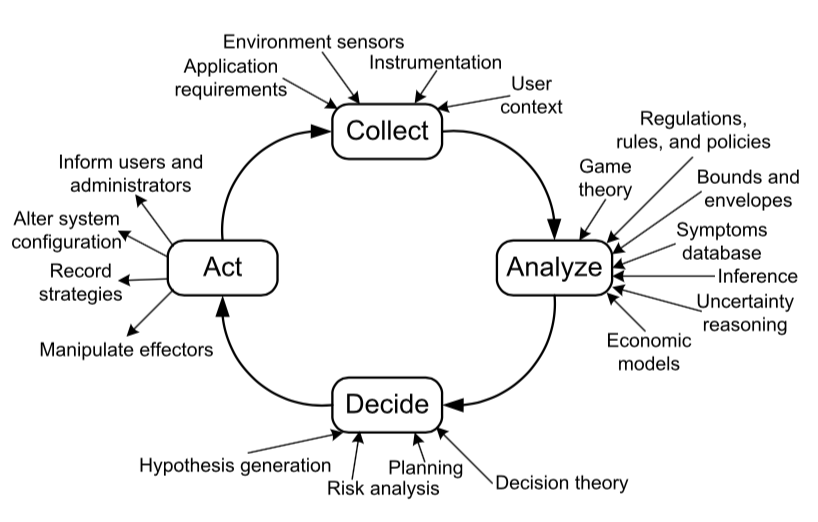
\includegraphics[width=0.8\textwidth]{imagens/generic-feedback-loop.png}
\caption{Ciclo de \textit{feedback} genérico \cite{dobson06}}
\label{generic-feedback-loop}
\end{figure}

Um exemplo da aplicação do clico de \textit{feedback} é discutido em \cite{brun09}. Os autores consideram que para manter os serviços Web em funcionamento durante um longo período de tempo requer a coleta de informações que reflitam o estado atual do sistema, analisando essas informações para diagnosticar problemas de desempenho ou para detectar falhas, decidindo como resolver o problema (por exemplo, via balanceamento dinâmico de carga ou corrigindo falhas), e agindo para efetuar as decisões tomadas.

Ao conceber um sistema adaptativo, algumas questões sobre essas atividades tornam-se importantes. Estas questões relativas aos laços de feedback devem ser explicitamente identificadas, registradas e resolvidas durante o desenvolvimento de um sistema adaptativo. A seguir serão apresentadas as questões levantas em \cite{brun09, lamprecht12}:

\begin{itemize}

\item O ciclo de \textit{feedback} começa com a coleta de dados relevantes de sensores disponíveis no ambiente e outras fontes que auxiliam na compreensão do estado atual do sistema. Algumas das questões que precisam ser respondidas aqui são: Qual é a taxa de amostragem necessária? Quão confiável é o dado do sensor? Existe um formato de evento comum entre os sensores? Os sensores fornecem informações suficientes para a identificação do sistema?;

\item Na sequência, o sistema analisa os dados coletados. Nesta etapa existem inúmeras abordagens para estruturar e raciocinar sobre os dados brutos (por exemplo, usando modelos, teorias e regras). Algumas das questões aplicáveis aqui são: Como o estado atual do sistema é inferido? Qual a quantidade/tempo de situações passadas podem ser necessárias no futuro? Quais dados precisam ser arquivados para validação, verificação e/ou conformidade? Quão fiel será o modelo ao mundo real e se um modelo adequado pode ser obtido a partir dos dados de sensores disponíveis? Quão estável será o modelo ao longo do tempo?;

\item Em seguida, uma decisão deve ser tomada para adaptar o sistema objetivando alcançar um estado desejável. Abordagens como análise de risco ajudam na escolha entre várias alternativas. Para esta atividade, as questões importantes são: Como o estado futuro do sistema é inferido? Como é alcançada uma decisão? Quais são as prioridades para a auto-adaptação em vários clicos de \textit{feedback} e em um único clico de \textit{feedback}?;

\item Finalmente, para implementar a decisão, o sistema deve agir por meio dos atuadores disponíveis. As questões importantes que surgem aqui são: Quando a adaptação deve e pode ser realizada com segurança? Como os ajustes de diferentes clicos de feedback interferem um ao outro? Os feedbacks centralizados ou descentralizados ajudam a atingir o objetivo global? Uma importante questão aplicável adicional é se o sistema de controle tem autoridade de comando suficiente sobre o processo, ou seja, se os atuadores disponíveis são suficientes para conduzir o sistema nas direções desejadas.

\end{itemize}

O modelo genérico de um clico de \textit{feedback} ilustrado na Figura \ref{generic-feedback-loop}, muitas vezes referido como o clico de controle autonômico, enfatiza as atividades que realizam feedback. Embora este modelo forneça um ponto de partida sobre os clicos de feedback, ele não detalha o fluxo de dados e o controle em torno do clico \cite{dobson06}. Ainda que esses clicos de feedback tenham tido muito sucesso em diferentes ramos de engenharia, como na teoria de controle, ainda não está claro se os princípios gerais desta disciplina podem ser aplicados diretamente em sistemas adaptativos. Diferentemente da teoria de controle, os cenários da IoT possuem uma estrutura não totalmente conhecida \cite{lamprecht12}.


Em uma tentativa de lidar com as complexidades dos sistemas modernos de computação a \textit{International Business Machines} (IBM) assumiu os desafios mencionados e sugeriu o modelo \textit{Monitor-Analyze-Plan-Execute plus Knowledge} (MAPE-K), conforme apresentado na Figura \ref{mape-k-model}. O MAPE-K utiliza as atividades Monitorar, Analizar, Planejar e Executar empregando um clico de controle em conjunto com o componente Conhecimento que fornece as informações necessárias para realizar a adaptação \cite{aman15}. O componente Monitor coleta os dados apropriados dos recursos gerenciados por meio dos sensores. Os dados são correlacionados, filtrados e/ou agregados e o sintoma descoberto é passado para o componente Analisar. Sintomas e outros dados também podem ser armazenados em uma base de conhecimento compartilhada. O analisador determina se uma mudança precisa ser feita com base no conhecimento compartilhado (potencialmente uma política) e nos sintomas. Caso pertinente, uma solicitação de mudança no ambiente é passada para o componente Planejar. O planejador gera os comandos ou fluxos de trabalho necessários na forma de um plano de alteração que é passado para o componente Executar. O executor aplica o plano de mudança no recurso de gerenciamento usando os atuadores. Caso necessário, a base de conhecimento pode ser atualizada, fornecendo dados do impacto da adaptação para serem aplicados como feedback para o próximo clico \cite{lamprecht12}.

\begin{figure}[ht]
\centering
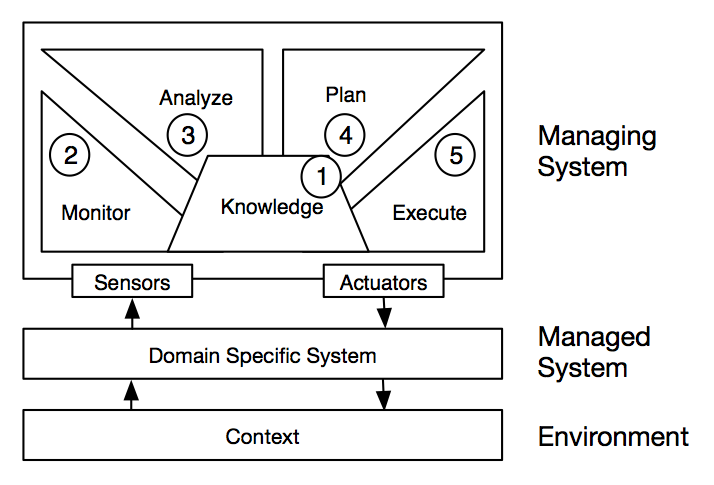
\includegraphics[width=0.8\textwidth]{imagens/mape-k-model.png}
\caption{MAPE-K - Modelo para sistema adaptativos \cite{iglesia15}}
\label{mape-k-model}
\end{figure}


De acordo com a IBM, um sistema autonômico deve ter os seguintes auto-atributos \cite{kephart03, iglesia15}: 

\begin{itemize}

\item Autoconfiguração (\textit{self-configuration}): o sistema deve se configurar automaticamente de acordo com as políticas de alto nível pré-definidas. Este atributo também contempla a facilidade de se adaptar às mudanças causadas por configurações automáticas. A integração, instalação e configuração de dispositivos e softwares devem ser feitos eficientemente. Caso a nova configuração não proporcione para a rede o desempenho esperado, há a possibilidade de restauração da mesma.

\item Auto-otimização (\textit{self-optimization}): consiste da habilidade do sistema controlar os recursos e os parâmetros de segurança para melhorar o desempenho e a eficiência, consequentemente aprimorando a qualidade dos serviços (QoS).

\item Autocura (\textit{self-healing}): é a capacidade do sistema detectar, diagnosticar e reparar falhas automaticamente sem que isto afete o funcionamento do sistema. A auto-cura é determinante na disponibilidade e confiabilidade do sistema.

\item Autoproteção (\textit{self-protection}): este atributo envolve dois aspectos: a defesa contra ataques e antecipação de ataques. A defesa deve ser realizada com o objetivo de protejer o sistema de ataques maliciosos ou falhas que não foram tratadas corretamente pela auto-cura. A antecipação de ataques é feita baseando-se em relatórios de sensores e, com essas informações, medidas devem ser adotadas para minimizar os problemas.

\end{itemize}

Em \cite{evesti13b}, os autores mencionam outros dois atributos, a autoconsciência (\textit{self-awareness}) e a ciência de contexto (\textit{context awareness}). A autoconsciência é a capacidade do sistema em conhecer seu próprio estado, seus componentes, capacidades, limites, recursos e comportamento. Já a ciência do contexto, consiste do conhecimento sobre o ambiente operacional ao qual o sistema está inserido. 


% gartner The Four Stages of an Adaptive Security Architecture???

%%%%%%%%%%%%%%%%%%%%%%%%%%%%%%%%%%%%%%%%%%%%%%%%%%%%%%%%%%%%%%%%%%%%%%%
\section{Ciência de Contexto na Segurança Adaptativa}

A ciência de contexto está presente nas pesquisas relacionadas a UbiComp, sendo um dos grandes desafios no desenvolvimento de aplicações nesta área.  Para entender o seu significado, primeiramente é necessário definir contexto, que de acordo com Dey (2001)\nocite{dey01} é qualquer informação que pode ser usada para caracterizar a situação de uma entidade (pessoa, local ou objeto) que é considerada relevante para a interação entre o usuário e a aplicação, incluindo o próprio usuário e a aplicação.

Contexto pode ser considerado também como uma descrição complexa de conhecimento compartilhado sobre circunstâncias físicas, sociais, históricas, entre outras, onde ações ou eventos ocorrem, percebendo assim a relação existente entre contexto e eventos. Contexto é o que contribui para a correta interpretação de uma ação ou evento, sem, no entanto, ser parte dessa ação/evento. Também pode ser considerado como sendo uma coleção de condições relevantes e influências que tornam uma situação única e compreensível \cite{brezillon99, li15}.

Existem seis questões básicas que podem ser realizadas para facilitar a compreensão do contexto, elas são conhecidas como 5W+1H \cite{vieira04}. No entanto, para determinadas aplicações algumas são mais importantes que outras. A seguir as seis questões são apresentadas:


\begin{itemize}

\item quem (\textit{who}): informação de presença e disponibilidade dos indivíduos no grupo, e de identificação dos participantes envolvidos num evento ou numa ação;

\item o quê (\textit{what}): informação sobre a ocorrência de um evento de interesse;

\item quando (\textit{when}): informação temporal sobre o evento, o momento em que o evento ocorreu;

\item onde (\textit{where}): informação espacial, de localização, o local onde o evento ocorreu;

\item por que (\textit{why}): informação subjetiva sobre as intenções e motivações que levaram à ocorrência do evento;

\item como (\textit{how}): informação sobre a maneira com que o evento ocorreu.

\end{itemize}

O contexto é relativo a um foco, onde foco pode ser uma tarefa ou um passo na resolução de um problema ou em uma tomada de decisão \cite{brezillon05}. Dessa forma, o foco determina onde está o contexto e o que pode ser considerado como importante, pois nem tudo que é contexto de uma situação é relevante para tal. 
 
As áreas da UbiComp e Inteligência Artificial foram as pioneiras nos estudos e utilização do conceito de contexto e, com isso, foram as que demonstraram o potencial da aplicação desse conceito nos sistemas computacionais. Ultimamente, a ciência de contexto vem sendo foco de um grande número de pesquisas dentro da UbiComp. Dessa forma, neste texto entende-se por ciência de contexto a capacidade de um sistema em usar o contexto para prover serviços e/ou informações relevantes para o usuário \cite{dey01}.

Ao se construir e executar aplicações ubíquas cientes de contexto há uma série de funcionalidades que devem ser providas, envolvendo desde a aquisição de informações contextuais, a partir do conjunto de fontes heterogêneas e distribuídas, até a representação dessas informações, seu processamento, armazenamento, e a realização de inferências para seu uso em tomadas de decisão \cite{bellavista12}. Tais tarefas se alinham ao clico de feedback empregado na formalização da segurança adaptativa.

Os sistemas cientes de contexto devem ser flexíveis, se adaptarem, e serem capazes de atuar automaticamente para ajudar o usuário na realização de suas atividades, o que está diretamente associado às necessidades das soluções para segurança da informação. Algumas motivações para usar a ciência de contexto são: 

\begin{itemize}

\item auxilia na compreensão da realidade;

\item facilita na adaptação de sistemas;

\item auxilia no processo de transformação dos dados em informação;

\item apoia a compreensão de eventos e de situações.

\end{itemize}

Em \cite{heimerl12},  é discutida a importância de contexto à segurança da informação. Inicialmente, ele defende a ideia de que informação sem contexto é simplesmente um dado, e não informação. Logo, dados são mais valiosos quando contextualizados.  Um cenário que exemplifica isto é apresentado em \cite{aman15}, onde é descrito um médico, atualmente em férias, usando seu smartphone. O mesmo recebe autorização por um Sistema de Controle de Acesso Baseado em Função, do inglês \textit{Role-Based Access Control} (RBAC), para acessar informações pessoais do paciente de um lugar incomum, em um fim de semana. Do ponto de vista do RBAC, esta atividade parece ser legítima, e o sistema deve conceder acesso. No entanto, se for analisado todo o contexto, isto é, o local incomum, o estado atual e a data de acesso, pode-se concluir que existe um risco envolvido se o acesso for concedido, ou seja, o smartphone pode ter sido comprometido. Portanto, para prover segurança adaptativa com eficiência deve-se avaliar a situação em um contexto holístico.

% Talvez colocar um outro exemplo
%\citealp{heimerl12} apresenta um exemplo, onde o autor considera uma solução de segurança relatando que o endereço IP 192.161.0.12 está passando por uma varredura de portas, no entanto, isto consiste simplesmente de uma parte dos dados. Ainda é  necessário descobrir o que esses dados significam ao analista de segurança, se seriam importantes ou somente ruído, logo, ele necessita identificar o contexto. Por exemplo, o alerta, que antes consistia apenas de um ``dado'' recebe um novo significado, o endereço IP 192.161.0.12 hipoteticamente pode ser o sistema que mantém o banco de dados dos cartões de créditos dos alunos de uma universidade, ou pode ser  um site interno que não tem valor real para a instituição.

%Embora, o contexto do alerta tenha sido aprimorado, ainda é possível supor que o servidor que está sendo atacado é chamado de ``sentinela'', e é um Windows Server 2008 R2 SP1, rodando Oracle 11g Enterprise, que está localizado em Pelotas, Rio Grande do Sul, Brasil, na linha 3 do \textit{data center}, prateleira A12, e que detém todos os registros de pacientes clínicos, abrangendo assim as normas \textit{Health Insurance Portability and Accountability Act} (HIPAA) e \textit{Health Information Technology for Economic and Clinical Health} (HITECH). Percebe-se que a contextualização dos dados é importante no processo de aquisição de informação, e que possui uma grande diferença na maneira como a informação é gerenciada e protegida, tornando-se relevante para segurança da informação.

No que tange a segurança adaptativa, caso os contextos relevantes para a identificação das situações a serem avaliadas não sejam adequadamente levadas em consideração, pode haver uma influência adversa no ambiente impactando nos serviços oferecidos. Observa-se que a segurança adaptativa, é fortemente dependente do ambiente monitorado e da visão holística sobre o mesmo. Em outras termos, a contextualização deve ocorrer em diferentes níveis arquiteturas (desde a coleta do evento, passando pela normalização, análise de risco e assim por diante). A ciência de contexto é especialmente crítica nos cenários da IoT, em particular na adaptação, pois esta consiste de uma comunicação máquina para máquina, a priori sem a inteligência (envolvimento direto) dos humanos. Caso sejam levados em consideração contextos irrelevantes, incorretos ou insuficientes, a adaptação pode não ser eficiente \cite{aman15}.



\section{Considerações sobre o Capítulo}

Inicialmente neste capítulo foi apresentada a definição de IoT, sendo destacado que a segurança adaptativa é considerado um desfio importante e atual. Posteriormente a segurança adaptativa foi discutida, sendo exposto que o uso de um clico de \textit{feedback} se faz necessário para apoiar a implantação deste conceito. Também foi descrito que a ciência de contexto é um atributo fundamental para a adaptação. Com isto, na seção seguinte foi analisada a ciência de contexto descrevendo como ela pode ser aplicada neste âmbito.


%%%%%%%%%%%%%%%%%%%%%%%%%%%%%%%%%%%%%%%%%%%%%%%%%%%%%%%%%%%%%%%%%%%%%%%
\chapter{Estado da Arte} 

Neste capítulo será apresentado o estado da arte das pesquisas que tem como tema processamento de eventos complexos e internet das coisas. Na seção seguinte será apresentado o protocolo seguido para a execução do mapeamento sistemático assim como todos os passos executados que levaram a escolha dos trabalhos de interesse. Por fim será apresentado uma discussão sobre as soluções abordadas nos trabalhos de interesse selecionados.    

\section{Mapeamento Sistemático da Literatura}

O mapeamento sistemático abordado neste capítulo é baseada na metodologia proposta por Petersen et al. (2008), onde seguindo a série de passos proposto, torna o estudo realizado, possível de ser replicado por outros pesquisadores \cite{petersen08}. A partir desta metodologia, podemos citar cinco etapas das quais serão seguidas por este mapeamento:

\begin{enumerate}
	\item Definição das questões de pesquisa;
	\item Execução da pesquisa para identificação de estudos primários realizados;
	\item Triagem inicial empregando critérios de inclusão e exclusão considerando o resumo dos artigos;
	\item Triagem final considerando as seções de introdução, concepção do projeto e conclusão;
	\item Extração dos dados e mapeamento.
	

\end{enumerate}  

Para a consulta dos trabalhos relacionados primeiramente foi definido um conjunto de palavras como candidatas a palavras chave para a String de busca, dentre estas podemos citar: \textit{internet of things}, \textit{distributed} e \textit{complex event processing}. A Partir da definição destas como palavras chave, foi possível elaborar a String de busca usada para executar as consultas sobre as bases da: ACM Digital Library, IEEE Explore, ScienceDirect, Springer, Web of Science e Scopus; e assim obter-se os trabalhos relacionados com o tema de pesquisa, as strings de consulta podem ser vistas na figura \ref{tab:stringBusca} incluindo a qual respectiva base estas foram executadas.



\begin{figure}[ht]
	\centering
	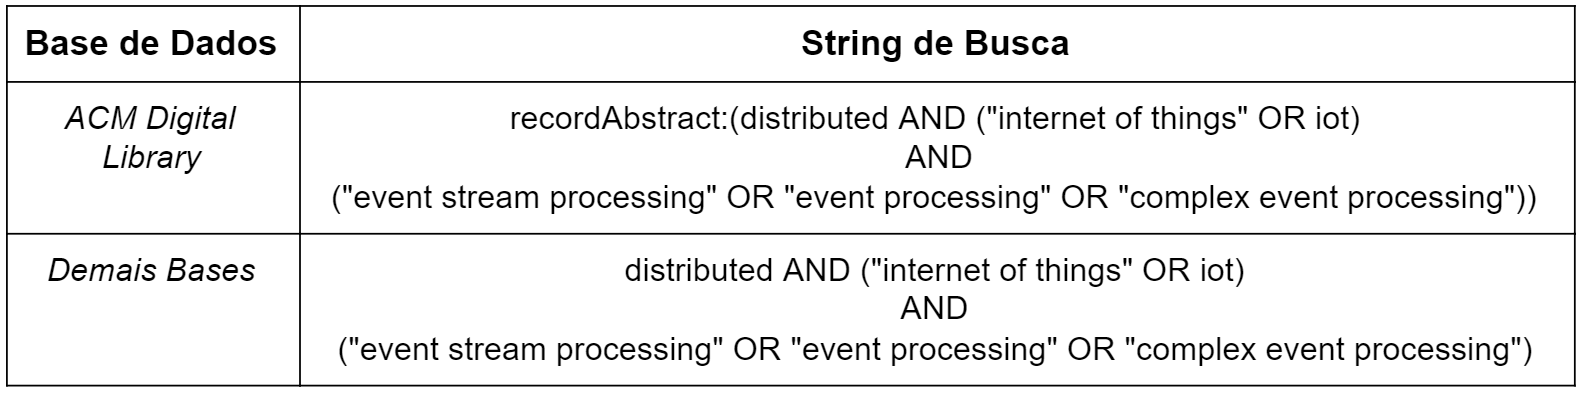
\includegraphics[width=1\textwidth]{imagens/tabela_string_busca.png}
	\caption{Strings de buscas usadas.}
	\label{tab:stringBusca}
\end{figure}

Após a execução desta consulta preliminar, que entende-se como a etapa de levantamento dos estudos primários relevantes, foi identificado 647 trabalhos de interesse onde este valor  compreende-se da soma dos resultados obtidos em todas as bases de consulta.

Todas as buscas foram realizadas sobre os metadados dos artigos(titulo, resumo e palavras chave), porem, como a base de dados Springer não oferecia suporte a este tipo de consulta, este problema foi contornado da seguinte forma: primeiramente foi feito a exportação do resultado preliminar da busca na base para o formato CSV(o único suportado) resultando em 472 artigos, após isto fez-se uso da ferramenta CSV2Bib\footnote{\url{https://github.com/jacksonpradolima/csv2bib}} para converter o arquivo CSV para bib com o intuito de importar o resultado, para a ferramenta Zotero\footnote{\url{http://lapes.dc.ufscar.br/tools/start_tool}}, que permitiu a execução da String de busca sobre os metadados dos 472 artigos encontrados preliminarmente, resultando em 6 documentos de interesse, a figura  \ref{fig:GrafBarraPubAno} apresenta um gráfico de barras contendo o numero de artigos encontrados pela String de busca em cada uma das bases, já o gráfico \ref{fig:GrafPizPubAno} apresenta o percentual de publicações que cada uma das bases contribuiu para o montante final.

\begin{figure}[ht]
	\centering
	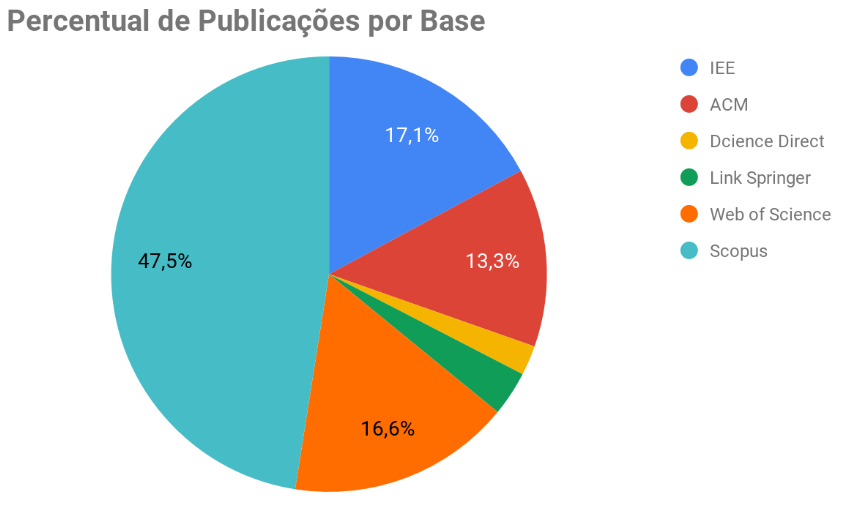
\includegraphics[width=.9\textwidth]{imagens/GrafPizPubAno.png}
	\caption{Percentual de publicações encontradas por base.}
	\label{fig:GrafPizPubAno}
\end{figure}

\begin{figure}[ht]
	\centering
	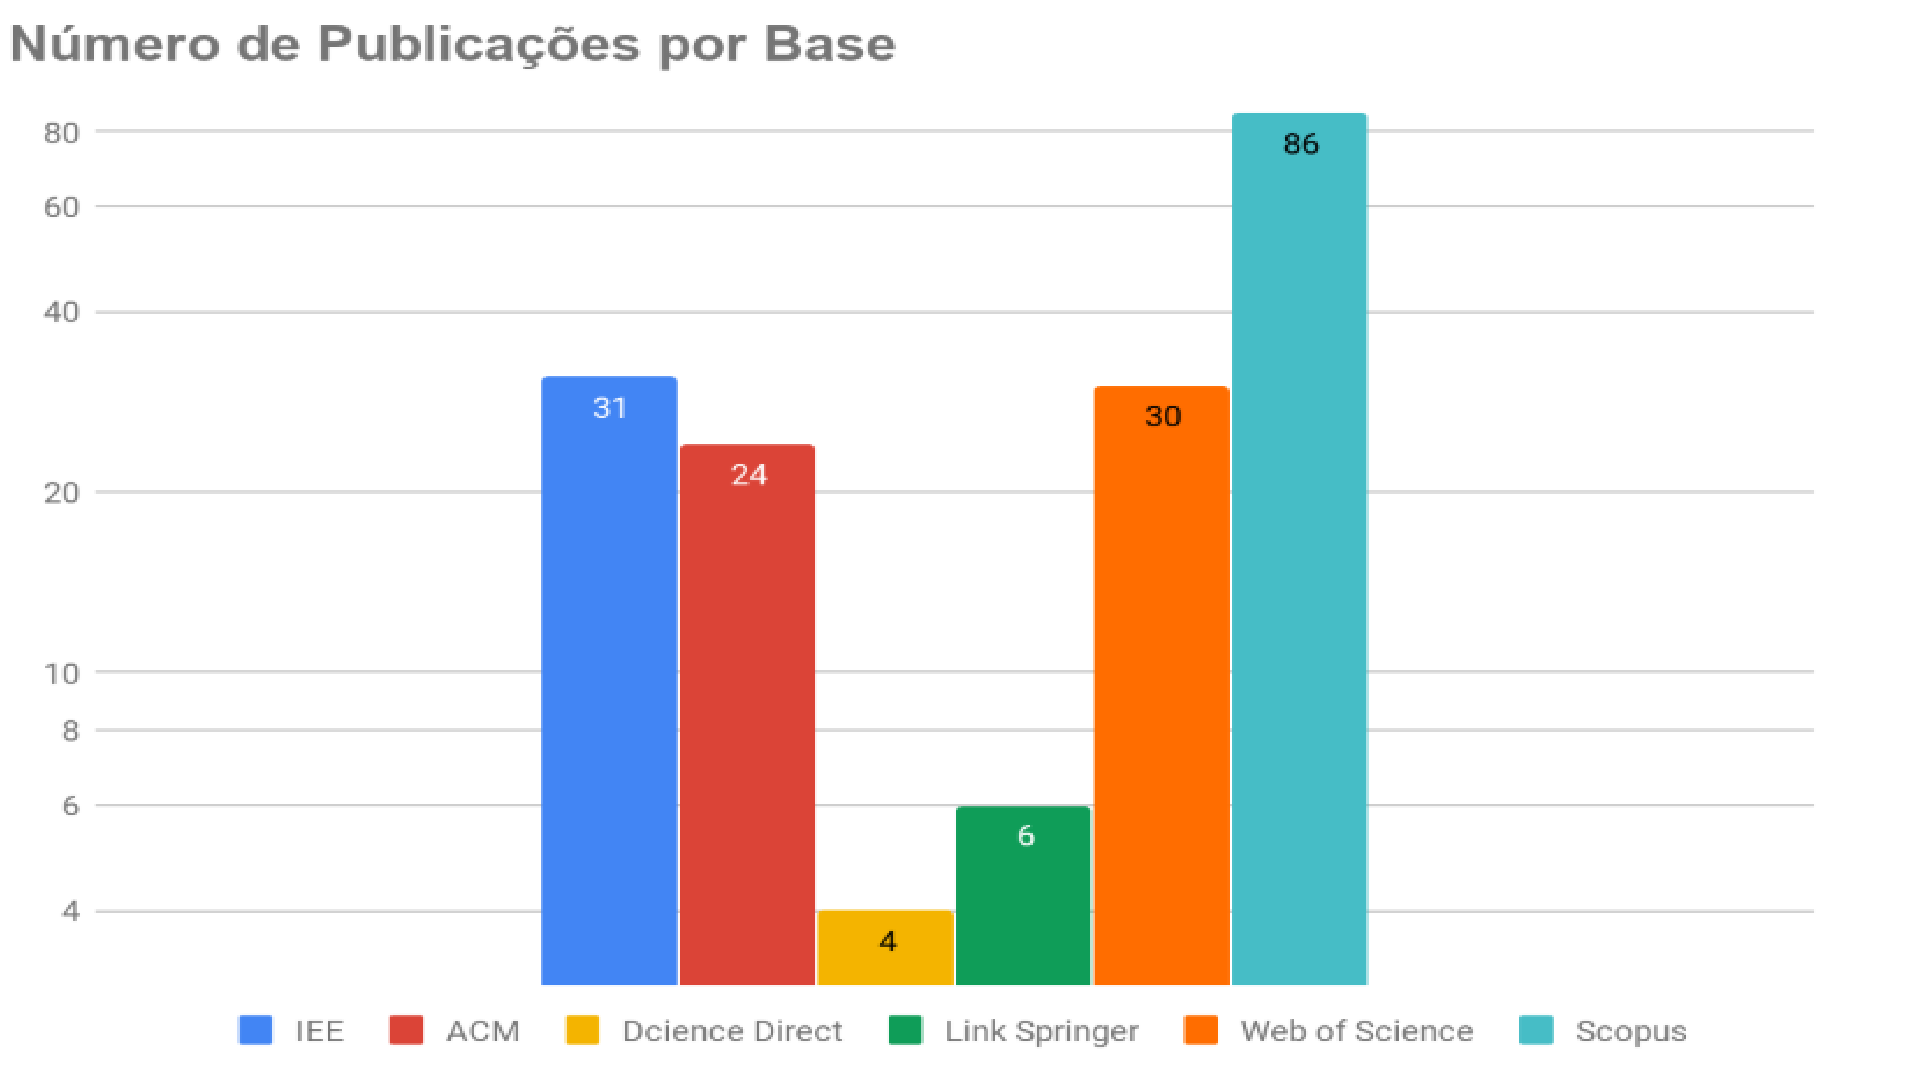
\includegraphics[width=.9\textwidth]{imagens/GrafBarraPubAno.png}
	\caption{Número de publicações encontradas por base.}
	\label{fig:GrafBarraPubAno}
\end{figure}


O gráfico \ref{fig:grafPublicaAno} apresenta o numero de publicações de interesse encontradas e cada uma das bases, o eixo X apresenta o ano do qual os artigos foram publicados e o eixo Y apresenta o numero total de publicações em relação ao ano, ainda podemos ressaltar que para a representação do gráfico foram removidos todas as publicações duplicadas. Podemos perceber pelo figura que a partir do ano de 2015 á uma ascendência no numero de publicações, e ainda um considerável pico no ano de 2017, demonstrando assim pontos de interesses neste período de publicações.

\begin{figure}[ht]
	\centering
	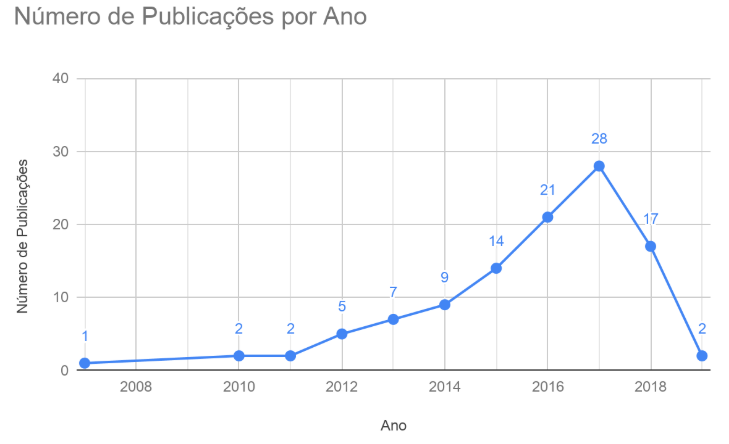
\includegraphics[width=.9\textwidth]{imagens/grafPublicaAno.png}
	\caption{Quantidade de publicações de interesse por ano.}
	\label{fig:grafPublicaAno}
\end{figure}

\subsection{Critérios de Inclusão e Exclusão}
Após a seleção inicial realizada sobre as bases de dados, executou-se a triagem inicial sobre o resumo dos artigos, aplicando os seguintes critérios de inclusão e exclusão conforme a ordem apresentada abaixo: 
\begin{itemize}
	\item (E) Foi publicado antes de 2015;
	\item (E) Não é um artigo Full paper;
	\item (E) Não esta em Inglês ou Português;
	\item (E) Indisponibilidade de acesso ao artigo completo;
	\item (E) Artigos que não tem prototipação;
	\item (E) Apresenta pequenas modificações de outro artigo;
	\item (I) Explora conceitos de segurança;
	\item (I) Explora conceitos de computação Ubiqua;
	\item (E) O artigo não possui nenhum dos critérios de inclusão.
\end{itemize}
	
Para auxiliar na aplicação dos critérios de inclusão e exclusão foi feita a importação dos resultados preliminares das buscas na ferramenta Start\footnote{\url{http://lapes.dc.ufscar.br/tools/start_tool}},
para isso usou-se os arquivos .bib exportados pelas ferramentas das bases de busca, com exceção apenas da Spriger, onde usou-se o arquivo .bib exportado pelo Zootero, que foi gerado apos a execução da consulta sobre os metadados, aplicada sobre o resultado preliminar da base.

Após execução da triagem inicial dos trabalhos, aplicando os critérios de inclusão e exclusão sobre o resumo dos artigos, selecionou-se 27 documentos de interesse. 

\section{Trabalhos Relacionados}

Como resultado do mapeamento sistemático da literatura foram selecionados 6 artigos, os quais são apresentados a seguir, sendo explorados aspectos referentes ao seu modelo, detalhes sobre o clico de \textit{feedback}, bem como, suas principais características. 


%%%%%%%%%%%%%%%%%%%%%%%%%%%%%%%%%%%%%%%%%%%%%%%%%%%%%%%%%%%%%%%%
\subsection{Risk-based Adaptive Security for Smart IoT in eHealth} % 2012

Este artigo propõem um \textit{framework} de segurança adaptativa baseado em risco para a IoT em cenários de \textit{eHealth} \cite{habtamu12}. O \textit{framework} é utiliza a teoria dos jogos e técnicas de ciência de contexto para estimar e prever o risco à segurança da informação. Os métodos e mecanismos de segurança do \textit{framework} buscam adaptar as decisões de segurança sobre essas estimativas e previsões. O \textit{framework} incorpora modelos de avaliação prática e sistemática que utilizam métricas de segurança para validação da adaptação.

A abordagem realiza um esforço para aumentar a segurança a um nível adequado, adaptando-se às condições dinâmicas de mudança da IoT, incluindo usabilidade, ameaças e heterogeneidade. O artigo também descreve um possível estudo de caso projetado para validação que propõem estratégias adaptativas para a interação dinâmica entre segurança e transmissão de dados em um sistema de monitoramento de pacientes móveis.

O \textit{framework} emprega o clico de controle adaptativo, por meio da metodologia \textit{Monitor-Analyze-Adapt}, para gerenciamento de riscos de segurança e privacidade levando em consideração as informações de contexto necessárias para garantir a eficiência ao longo do tempo. A Tabela \ref{aligment-iso-27005} mostra o alinhamento da metodologia Plan-Do-Check-Act (PDCA) apresentada na ISO/IEC 27005:2008 com os processos \textit{Information Security Management System} (ISMS) e \textit{Information Security Risk Management} (ISRM) com a \textit{Adaptive Risk Management} (ARM) proposta.

        \begin{table}[h]
        \centering
	\caption{Alinhamento da ISO/IEC 27005 ISMS, ISRM e ARM}
	\label{aligment-iso-27005}
	\begin{tabular}{p{2cm}|p{6cm}|p{6cm}}
	\rowcolor[HTML]{003366}
	\textcolor{white}{\textbf{Processo ISMS}} & \textcolor{white}{\textbf{Processo ISRM}} & \textcolor{white}{\textbf{Processo/Metodologia ARM Proposto}} \\
	\hline
	\cellcolor[HTML]{E5EAEA} \textbf{\textit{Plan}} & \textit{Establish the context; Risk assessment; Risk treatment planning; Risk acceptance} & \textit{Analyze (plan): establish security} \\
	\hline
	\cellcolor[HTML]{E5EAEA} \textbf{\textit{Do}} & \textit{Implementation of risk treatment plan} & \textit{Adapt (Execute): adapt, implement and operate security} \\
	\hline
	\cellcolor[HTML]{E5EAEA} \textbf{\textit{Check}} & \textit{Continual monitoring and reviewing of risks} & \textit{Monitor: monitor and review security} \\
	\hline
	\cellcolor[HTML]{E5EAEA} \textbf{\textit{Act}} & \textit{Maintain and improve the ISRM process} & \textit{Adapt (learn): maintain, learn \& improve security}
	\end{tabular}
	\end{table}

Os autores definem como ARM um modelo de gerenciamento de riscos capaz de aprender, adaptar, prevenir, identificar e responder a ameaças conhecidas e desconhecidas em tempo real. A principal função deste modelo é o desenvolvimento de métodos e mecanismos de segurança adaptativos baseados em risco para dispositivos inteligentes da IoT que estimam e prevêem danos de risco e benefícios futuros, integrando modelos de monitoramento adaptativo, analítico e preditivo, modelos de decisão adaptativa e modelos de avaliação e validação em um ciclo contínuo, permitindo que os métodos e mecanismos de segurança adaptem suas decisões sobre essas estimativas e previsões.

Para enfrentar esses desafios, o modelo ARM proposto considera as seguintes medidas necessárias: (i) identificação - capacidade de prever problemas, (ii) análise - capacidade de prever o impacto, (iii) planejamento para implementar ações planejadas, (iv) rastreabilidade - capacidade de manter o foco do gerenciamento em ações de mitigação de risco, e (v) controle - capacidade de reduzir a exposição ao risco. Estas medidas são alcançadas através da coordenação de diferentes modelos.

A Figura \ref{adaptive-security-management-model} descreve o framework de segurança adaptativa baseada em risco para a IoT. O framework consiste em (i) o modelo de gerenciamento de risco adaptativo, (ii) o modelo de monitoramento adaptativo, (iii) os modelos analíticos e preditivos, (iv) os modelos adaptativos de tomada de decisão e (v) os modelos de avaliação e validação.

\begin{figure}[ht]
\centering
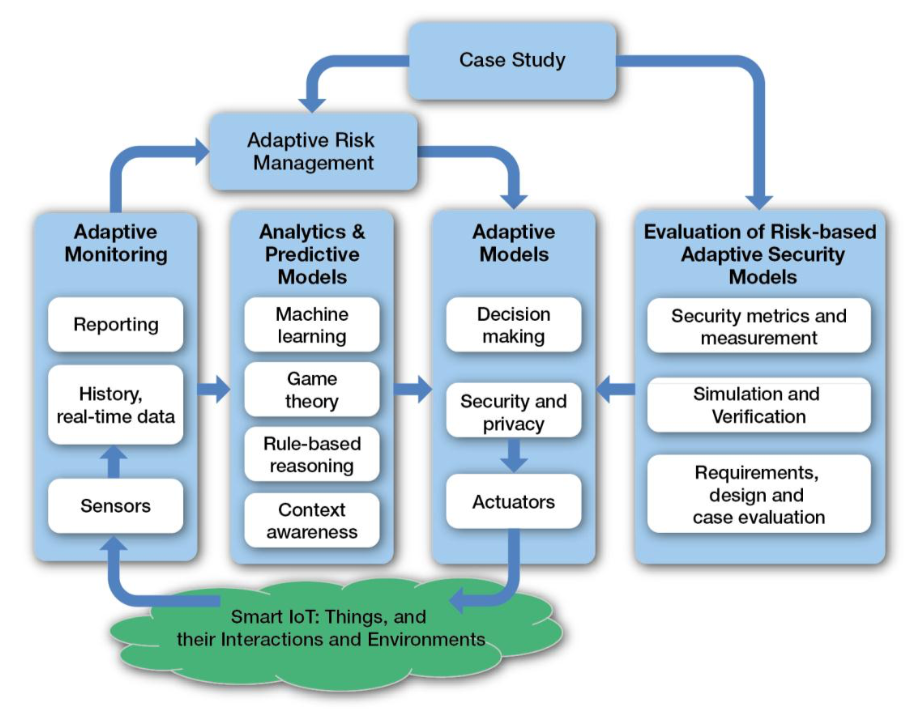
\includegraphics[width=0.7\textwidth]{imagens/adaptive-security-management-model.png}
\caption{Modelo proposto para gerenciamento de segurança adaptativa}
\label{adaptive-security-management-model}
\end{figure}

O modelo de monitoramento de segurança adaptável (\textit{Adaptive Monitoring}) empregado no framework foi proposto pelos autores em \cite{abie10} e é utilizado para obter evidências técnicas automatizadas para fins de monitoramento de segurança operacional contínua. O modelo de monitoramento de segurança adaptável adapta a arquitetura seguindo um ciclo contínuo de monitoramento das informações de contexto e estado dos dispositivos inteligentes da IoT que são explorados em tempo de execução no processo de adaptação.

Os modelos analíticos e preditivos analisam as informações coletadas  a partir do modelo de monitoramento adaptativo usando a teoria dos jogos e a ciência de contexto para estimar e prever dinamicamente riscos de segurança e privacidade e benefícios futuros, visando compreender e priorizar as atividades de tomada de decisão e analisar a segurança socioeconômica da segurança adaptativa na IoT. A teoria dos jogos foi escolhida pois pode modelar o comportamento dinâmico das partes interessadas com interesses conflitantes, incluindo as estratégias dos adversários do mundo real. Os modelos também buscam aprimorar a precisão das estimativas aplicando métodos de aprendizado automatizado e algoritmos baseados em regras.

Na eHealth baseada na IoT, segurança adaptativa para tomada de decisão é necessária para adaptar os meios de proteção dos dispositivos envolvidos, suas interações e seu ambiente contra intrusos maliciosos e usuários autorizados. O modelo de tomada de decisão adapta-se ao dinamismo desses dispositivos, suas interações, ao meio ambiente e aos diversos graus de risco que o sistema da IoT para eHealth será confrontado. Isso é realizado determinando dinamicamente se as mudanças e a adaptação devem ser feitas ou não e, se for feita, selecionando o ``melhor'' modelo de segurança adaptativo para uma determinada situação para posteriormente aplicar as mudanças e adaptações identificadas garantindo a maior probabilidade de alcançar o maior benefício para o menor risco. O modelo geral de tomada de decisão adaptativa também aprende e se adapta a um ambiente de IoT em mudança em tempo de execução. Isso é feito (i) combinando modelos adaptativos de decisão baseado em risco, modelos adaptativos de segurança e privacidade e atuadores para fazer uma reação adaptativa efetiva, e (ii) integrando diferentes métricas para validação e verificação, avaliação adaptativa de risco e modelos de análise preditiva para estimativa e previsão de riscos e impactos de segurança e privacidade.


Medições de segurança e métricas são necessárias para avaliar e validar de forma mensurável a adaptação em tempo de execução. As técnicas de decomposição de objetivos de segurança são promissoras e evoluirão com modelos teóricos e matemáticos para medir e validar o potencial dos modelos de segurança adaptativa para IoT. As técnicas permitem capturar requisitos e métricas de projeto em diferentes níveis de abstração para determinar e identificar lacunas e obstáculos nos níveis de arquitetura e modelo. As métricas de segurança baseadas em simulação preditiva e verificação podem auxiliar a entender as diferentes soluções, variando os pressupostos sobre ameaças e requisitos, para selecionar métricas que servem como indicadores de riscos de segurança para a IoT.


O artigo detalha ainda um possível estudo de caso baseado no fato de que os sistemas de monitoramento de pacientes são uma importante fonte de dados em ambientes de saúde. É ressaltado que esses sistemas devem manter um certo nível de disponibilidade, QoS, segurança e proteção de privacidade do paciente. Com isso, os autores apresentam um estudo de caso (vide Figura \ref{case-study-patient-monitoring}) baseado em um sistema de monitoramento de pacientes apoiado pela IoT . O paciente pode estar em casa ou no hospital, e os dispositivos da IoT incluem \textit{smartphones}, \textit{tablets}, sensores e atuadores.

\begin{figure}[ht]
\centering
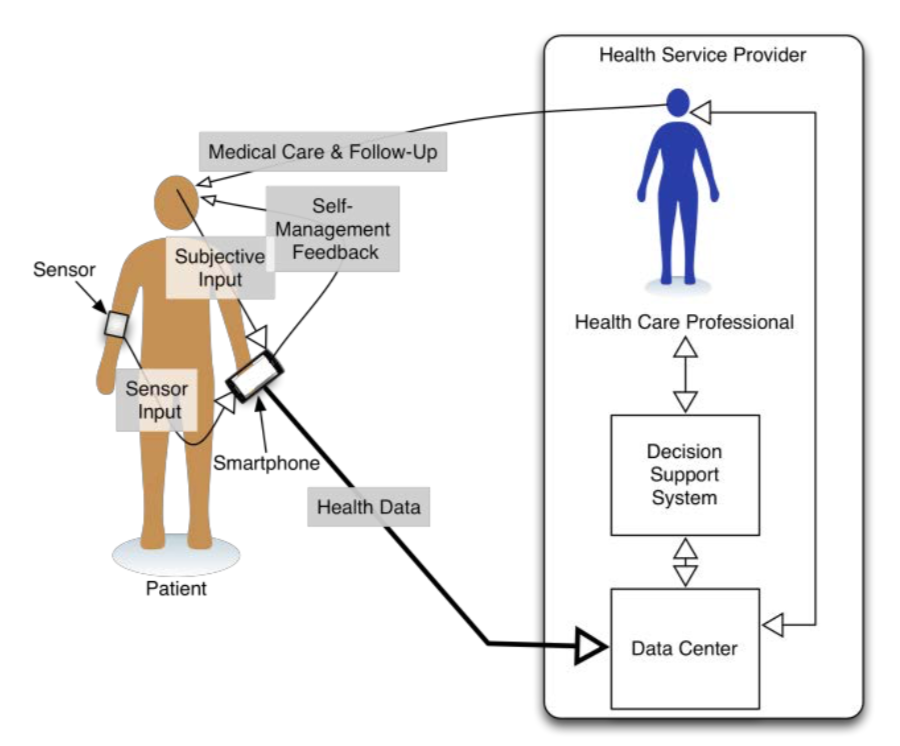
\includegraphics[width=0.7\textwidth]{imagens/case-study-patient-monitoring.png}
\caption{Estudo de caso baseado em monitoramento de paciente}
\label{case-study-patient-monitoring}
\end{figure}


Como trabalho futuro os autores destacam o desenvolvimento e prototipação dos modelos para estimar e prever riscos e benefícios usando a teoria dos jogos e a ciência de contexto, definir a metodologia para medições de segurança e métricas para validar a eficácia da adaptação, bem como conceber dispositivos inteligentes com mecanismos de baixo consumo de recursos que irão permitir a detecção de ameaças em tempo de execução, respondendo a elas e se adaptando ao meio ambiente aprimorando o grau de segurança e privacidade. Também é incluído a necessidade de validação do cenário proposto.


%%%%%%%%%%%%%%%%%%%%%%%%%%%%%%%%%%%%%%%%%%%%%%%%%%%%%%%%%%%%%%%%

\subsection{Architecture and Knowledge-Driven Self-Adaptive Security in Smart Space} % 2013

Este artigo apresenta uma arquitetura para segurança adaptativa em espaços inteligentes. A abordagem combina um ciclo de adaptação, uma ontologia denominada \textit{Information Security Measuring Ontology} (ISMO) e um modelo de controle de segurança para espaços inteligentes. O ciclo de adaptação inclui as fases de monitoramento, análise, planejamento e execução de mudanças no espaço inteligente. De acordo com os autores, a abordagem se diferencia por definir todo o ciclo de adaptação e o conhecimento necessário em cada etapa. As contribuições são validadas como parte do protótipo de um espaço inteligente. A abordagem oferece meios reutilizáveis e extensíveis para alcançar a segurança adaptativa em espaços inteligentes \cite{evesti13c}. 

Apesar de neste artigo a arquitetura ser explorada por meio de políticas dinâmicas de controle de acesso, o trabalho foi extendido em \cite{evesti13a}, onde outros cenários de uso são expostos. Ou seja, a segurança adaptativa pode ser aplicada em vários domínios, sendo uma abordagem de adaptação genérica, consequentemente permitindo a adaptação à vários objetivos de segurança. Além disso, a abordagem deve aplicar os mecanismos de segurança existentes, em vez de desenvolver mecanismos dedicados para fins de adaptação.

A estrutura da arquitetura proposta é apresentada na Figura \ref{ismo-architecture}, onde observa-se que a mesma está em conformidade com o modelo de referência MAPE-K. Consequentemente, os componentes \textit{Monitor}, \textit{Analyser}, \textit{Planner} e \textit{Executor} desempenham um papel fundamental na estrutura, ou seja, a arquitetura aplica o ciclo de adaptação MAPE completo para a segurança adaptativa e define cada fase separadamente. O conhecimento é oferecido a partir da ontologia no formato \textit{Ontology Web Language} (OWL), a ISMO, a qual está conectada aos componentes \textit{Monitor}, \textit{Analyser} e \textit{Planner} que utilizam o seu conhecimento.

\begin{figure}[ht]
\centering
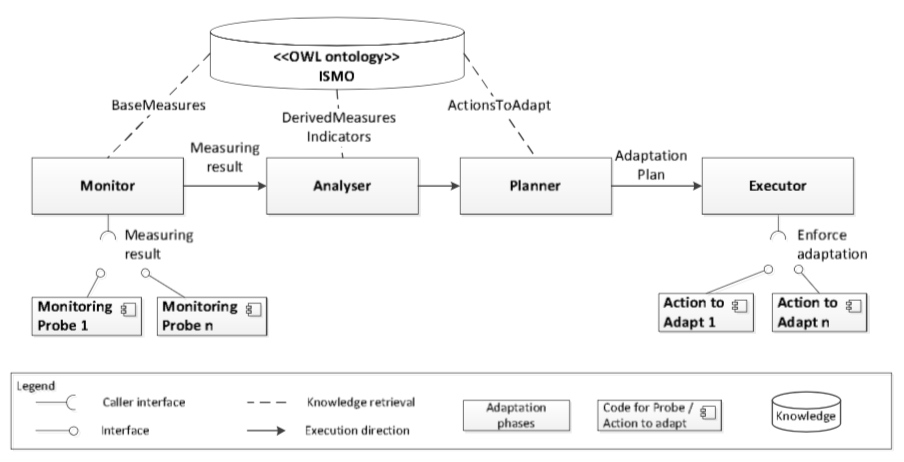
\includegraphics[width=0.7\textwidth]{imagens/ismo-architecture.png}
\caption{Estrutura da arquitetura de adaptação}
\label{ismo-architecture}
\end{figure}

O componente \textit{Monitor} está conectado aos componentes \textit{Monitoring Probe}, ao \textit{Analyzer} e ao ISMO. Da ISMO, o \textit{Monitor} recupera as métricas base. Assim, apenas as métricas para os objetivos de segurança exigidos e os mecanismos de segurança utilizados são usadas. Cada métrica base possui sua própria abordagem de medição que descreve como realizar a medição. Os componentes \textit{Monitoring Probe} são trechos de código que implementam os métodos de medição. O componente \textit{Monitor} solicita a medição dos resultados dos componentes \textit{Monitoring Probe} selecionados. A solução proposta utiliza métricas de segurança para monitorar o nível de segurança alcançado. 

O componente \textit{Analyzer} é chamado pelo componente Monitor. A Figura \ref{ismo-monitor} mostra os componentes internos do componente  \textit{Analyzer} para calcular o indicador de nível de segurança. O \textit{Analyzer} recupera medidas derivadas, indicadores e abordagens de medição relacionadas da ISMO. O componente analisa as regras dos modelos de análise que são utilizados no componente do combinador de métricas base (\textit{Base measure combiner}) para calcular o indicador de nível de segurança. Posteriormente, o componente \textit{Analyzer} compara os níveis de segurança alcançados e necessários com base em informações contextuais monitoradas e chama o componente \textit{Planner} se a segurança necessária não tiver sido alcançada. 


\begin{figure}[ht]
\centering
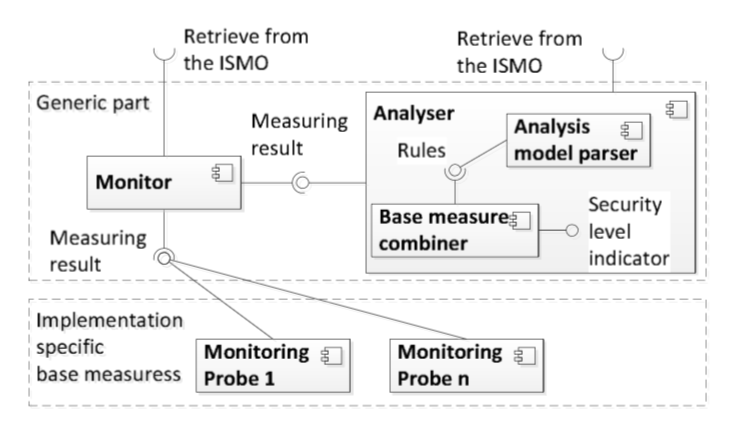
\includegraphics[width=0.7\textwidth]{imagens/ismo-monitor.png}
\caption{Partes genéricas e específicas da implementação do monitoramento do nível de segurança}
\label{ismo-monitor}
\end{figure}

O objetivo do componente Planner é criar um plano de adaptação. O componente é conectado à ontologia ISMO para recuperar mecanismos ou atributos de segurança alternativos para alcançar a segurança necessária. O plano de adaptação é definido em tempo de modelagem e decidido em tempo de execução com base no conhecimento da ISMO, ou na pior situação, as instruções sobre como proceder são solicitadas ao usuário.

O \textit{Executor} é o último componente no loop de adaptação. Seu objetivo é fazer cumprir o plano de adaptação recebido como entrada do componente \textit{Planner}. Assim, ele está conectado aos componentes \textit{Action to Adapt}, que são implementações para adaptar a segurança, ou seja, são mecanismos de segurança destinados a aplicar ou modificar os atributos dos mecanismos de segurança.

No que diz respeito a base de conhecimento ISMO, é ressaltado que a adaptação de segurança requer: i) conhecimento de segurança, ii) medição de conhecimento e iii) conhecimento de contexto. O conhecimento de segurança define objetivos de segurança, mecanismos, ameaças e como eles estão relacionados. Posteriormente, a medição do conhecimento descreve os atributos e a forma de medi-los. Por último, o conhecimento de contexto descreve o espaço inteligente e o papel dos dados, usuários e ações dentro do espaço inteligente. Essas três áreas de conhecimento são apresentadas na Figura \ref{ismo-ontology}.

\begin{figure}[ht]
\centering
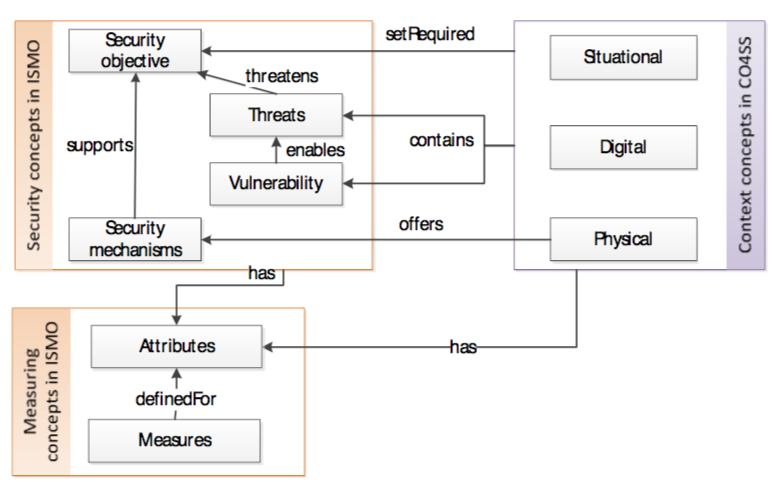
\includegraphics[width=0.7\textwidth]{imagens/ismo-ontology.png}
\caption{Dependências entre ontologias de segurança e de contexto}
\label{ismo-ontology}
\end{figure}


Como contribuições, o trabalho apresentou dois casos de uso da ontologia aplicada em tempo de modelagem e em tempo de execução. É também destacado a possibilidade de reuso e extensão tanto da ontologia quanto da arquitetura para adaptações de segurança, a qual contempla todas as fases do modelo MAPE-K. Finalmente, os autores enfatizam o fato de esta ser a primeira arquitetura até o momento da sua publicação que apresentou uma separação entre a base de conhecimento do ciclo de adaptação. 

%%%%%%%%%%%%%%%%%%%%%%%%%%%%%%%%%%%%%%%%%%%%%%%%%%%%%%%%%%%%%%%%

\subsection{Event driven adaptive security in internet of things} % 2014

Em \cite{aman14}, o objetivo dos autores é a concepção de uma solução autônoma para o gerenciamento de risco adaptativo para a IoT que possa analisar situações adversas em um contexto distinto e gerenciar o risco envolvido de forma inteligente para que as preferências do usuário final, o serviço e a segurança  estejam preservadas. Com isto, o artigo detalha o modelo de segurança adaptativa orientada a eventos para IoT e explica como ele pode ser aplicado em um cenário de eHealth para proteger o ambiente de ameaças em tempo de execução.

Os autores destacam a ausência de um modelo com métodos específicos para abordar e conectar análises e adaptações como uma solução holística. Por isso, eles exploram essa problemática como um conjunto de duas questões: como monitorar e coletar mudanças de segurança em tempo de execução e analisá-las em um contexto específico, e; como as informações analisadas podem ser usadas para adaptar configurações de segurança, de modo que as preferências de usuários e serviços sejam preservadas.
 
A primeira questão é abordada utilizando a solução \textit{Open Source Security Information Management} (OSSIM) \cite{ossim18}, que fornece uma plataforma para escrever \textit{scripts}, chamados de \textit{plugins}, para filtrar e normalizar eventos primitivos de segurança coletados de diferentes dispositivos presentes no escopo monitorado. As diretivas de correlação do OSSIM são especificadas por meio de regras em \textit{eXtensible Markup Language} (XML) para modelar situações adversas em que eventos de segurança são correlacionados e analisados, em uma visão temporal e espacial, considerando um contexto particular. 


A segunda questão é tratada por meio de uma ontologia proposta para adaptação que aproveita as informações de risco da correlação de eventos e adapta as configurações de segurança em tempo de execução. A ontologia permite que uma ação de mitigação seja selecionada de um conjunto de ações de forma que sua utilidade, em termos de usabilidade, QoS e confiabilidade de segurança, seja máxima entre as possíveis ações conforme os requisitos do usuário.

A principal contribuição deste artigo é a ontologia de adaptação autonômica à segurança. A OSSIM não fornece essa capacidade e depende de reconfigurações manuais que podem não atender aos requisitos do usuário e do serviço. Além disso, o OSSIM está focado no ambiente de computação tradicional, incluindo servidores, desktops e aplicações correspondentes, onde o processamento de eventos é relativamente uma tarefa comum. Este artigo amplia a segurança orientada à eventos para a IoT, onde o ambiente se torna mais complexo devido à diversidade e mobilidade dos dispositivos para as quais os protocolos e ferramentas tradicionais são ineficientes para processar eventos.

O modelo apresentado, \textit{Event Driven Adaptive Security} (EDAS), aborda a segurança adaptativa na IoT como uma \textit{Event Driven Architecture} (EDA) na forma de um clico de \textit{feedback}. O elemento básico de mudança disponível no ambiente monitorado é o evento gerado por várias aplicações e dispositivos registrados em arquivos de log. Eles fornecem um contexto primitivo sobre ``quem, quando, onde e o que'' provoca uma mudança e contém informações importantes, como data, origem, destino, atividade do usuário, níveis de gravidade, entre outras, necessárias para detectar situações de risco associadas a um evento. Um modelo de referência é apresentado na Figura \ref{edas-reference-model}, a qual inclui três principais componentes \textit{Monitor}, \textit{Analyzer} e \textit{Adaptor}.

\begin{figure}[ht]
\centering
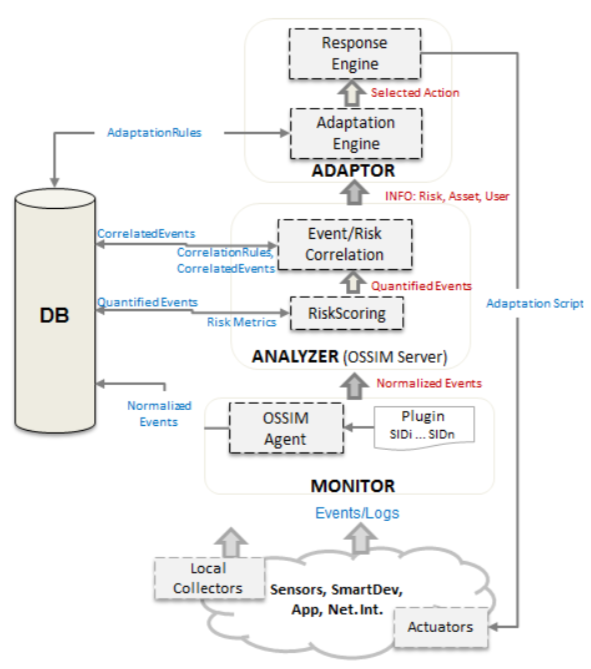
\includegraphics[width=0.7\textwidth]{imagens/edas-reference-model.png}
\caption{EDAS - modelo de referência}
\label{edas-reference-model}
\end{figure}

O componente \textit{Monitor}, prototipado por meio do OSSIM Agent, coleta, filtra e normaliza eventos de diferentes dispositivos da IoT. Para a coleta, o EDAS faz uso tanto da bordagem com agente quanto sem agente (conhecida como \textit{agent-less}), neste caso explorando protocolos como Syslog e SNMP. No que diz respeito aos dispositivos da IoT, os autores adotaram um agente baseado no \textit{MQ Telemetry Transport} (MQTT), um protocolo de transporte de mensagens \textit{Machine-To-Machine} M2M projetado especificamente para IoT independente de plataforma. O cliente do MQTT conecta-se à API de eventos do dispositivo para coletar eventos de segurança gerados e os transporta para o OSSIM Agent, onde eles são armazenados em um arquivo de log específico.

A filtragem de eventos é realizadas através dos \textit{plugins}, concebidos para fontes de eventos individuais. Escrever estes \textit{plugins} requer algum conhecimento da fonte e dos eventos que estão sendo analisados. O \textit{plugin}, identificado por um ID exclusivo e outros parâmetros necessários, é um arquivo de configuração que determina quais eventos da fila devem ser tratados e quais deles precisam ser filtrados. A OSSIM utiliza um mecanismo de lista branca (do inglês \textit{white-listing}) baseado em expressões regulares onde apenas eventos de interesse são enviados para posterior processamento. Quando ocorre uma correspondência com as expressões um identificador único de segurança (SID) é atribuído ao evento, o qual é geralmente utilizado na correlação de eventos.

A normalização é realizada pois diferentes dispositivos da IoT produzem eventos em diferentes formatos. Logo, é necessário transformá-los em um único formato comum para correlação e análise. Este processo é realizado durante a extração de SIDs e visa também extrair atributos importantes de um evento. Os atributos variam de evento para evento dependendo do contexto primitivo que eles possuem.

O componente \textit{Analyzer} é prototipado por meio do OSSIM Server. Inicialmente, antes dos eventos serem correlacionados, uma pontuação de risco é atribuída à eles. A OSSIM usa três métricas para calcular o risco do evento em tempo de execução:

\begin{itemize}
\item Valor do ativo (\textit{asset value}): determina a importância da origem ou do destino dos eventos dentro do escopo monitorado. Varia de 0 a 5.
\item Prioridade (\textit{priority}): especifica o impacto do evento. Varia de 0 a 5.
\item Confiabilidade (\textit{reliability}): determina a probabilidade ou a confiança de que o evento corresponderá a um comprometimento do ativo. A confiabilidade varia entre 0-10.

\end{itemize}

Com isto, para cada evento X o risco é quantificado na função:

\begin{center}
\begin{math}
Risk(X) = (Priority \times AssetV alue \times Reliability)/25 
\end{math}
\end{center}

A divisão de 25 é feita para manter os valores de risco no intervalo de 0 a 10, o que reflete o nível de risco de cada evento. Esses valores são atribuídos à medida que chegam no mecanismo \textit{Risk Scoring}, e são armazenados no banco de dados mantendo a relação com cada SID, podendo ser alterados manualmente conforme necessário. Já os valores de prioridade e confiabilidade podem ter valores diferentes configurados nas diretivas de correlação.

Na sequência, o mecanismo de correlação analisa os eventos usando diretrizes de correlação armazenadas em XML. A correlação é disparada quando um SID específico é encontrado e, portanto, um novo evento é gerado com um novo valor de confiabilidade. O motor aumenta e diminui esse valor com os respectivos atributos definidos dentro das diretivas. Portanto, o risco é avaliado dinamicamente quando os SIDs são correlacionados ao longo do tempo. A correlação de eventos produz eventos de alto nível que vão para uma correlação detalhada ou são marcados como alarmes a serem gerenciados. Os alarmes são eventos correlacionados com o nível de risco acima do limite de aceitação de risco. As informações carregadas por um alarme incluem IDs de origem e de destino, o usuário envolvido, o nível de risco, os detalhes da ameaça e a diretiva de correlação responsável por gerá-lo. Esta informação é utilizada durante o processo de adaptação onde o risco confrontado é mitigado.

Para utilizar o conhecimento disponível de forma precisa e adaptar as configurações de segurança de forma otimizada, a ontologia de adaptação proposta é empregada. Para operar em tempo de execução, a ontologia considera todas as entidades e seus relacionamentos necessários para uma segurança adaptativa otimizada. O modelo proposto é utilizado em um cenário de \textit{eHealth} habilitado para IoT, onde um paciente é gerenciado remotamente pela internet ou rede celular. Para isso, três contextos diferentes foram estabelecidos na ontologia proposta, conforme mostrado na Figura \ref{edas-ontology}.

\begin{figure}[ht]
\centering
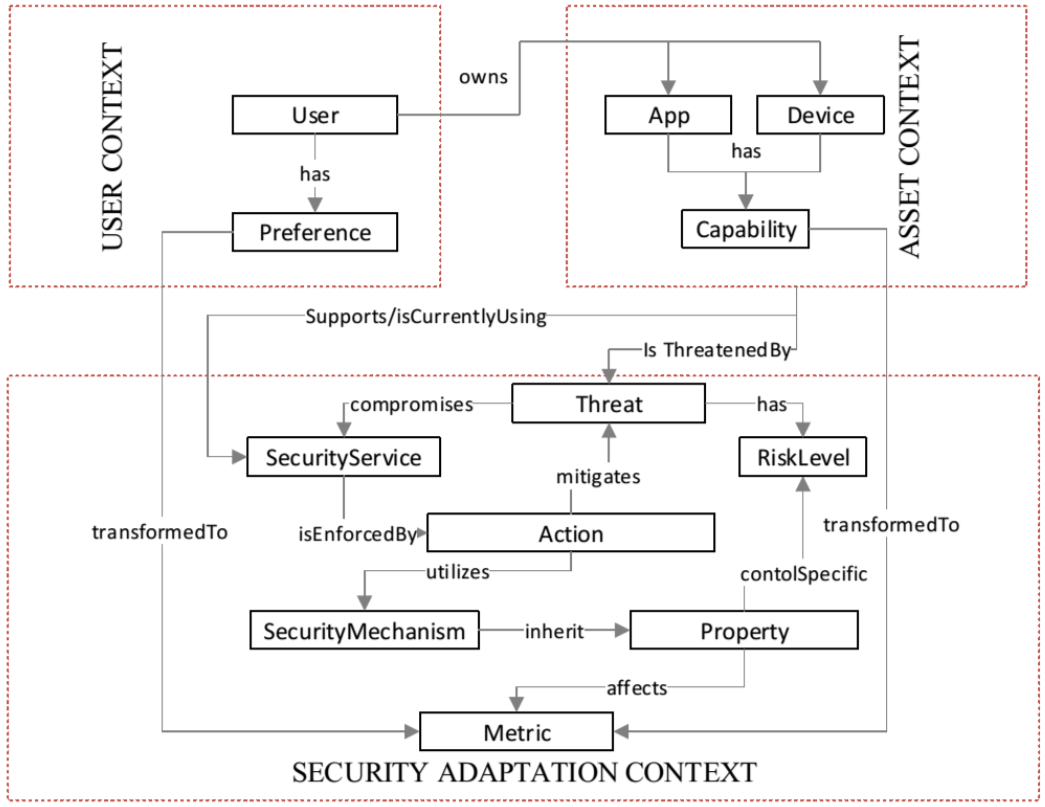
\includegraphics[width=0.7\textwidth]{imagens/edas-ontology.png}
\caption{EDAS - ontologia para segurança adaptativa}
\label{edas-ontology}
\end{figure}


O \textit{User Context} corresponde às preferências do paciente e da equipe médica que devem ser consideradas antes da adaptação Cada usuário possui ou utiliza um conjunto de aplicativos, como o aplicativo \textit{eHealth}, o Skype para comunicação paciente-médico, entre outros, e dispositivos, como sensores corporais, dispositivos inteligentes ou \textit{desktop}/notebook, no escopo da infraestrutura da IoT-eHealth. As informações correspondentes, por exemplo, tipo, valor de ativos, etc., juntamente com suas capacidades, estão contidas em \textit{Asset Context}. As entidades e as configurações associadas necessárias para a adaptação de segurança otimizada são agrupadas no \textit{Security Adaptation Context}.

Uma ação de mitigação ideal é selecionada a partir do conjunto de ações seguindo o procedimento mostrado na Figura \ref{edas-adaptation-process}. O mecanismo de resposta (\textit{Response engine}) envia uma mensagem usando o MQTT para um atuador (cliente MQTT instalado no dispositivo monitorado) com os detalhes da ação fornecida pelo mecanismo de adaptação. O atuador é conectado à API do dispositivo, por exemplo uma API de autenticação, e encaminha a mensagem como variáveis a serem reconfiguradas.

\begin{figure}[ht]
\centering
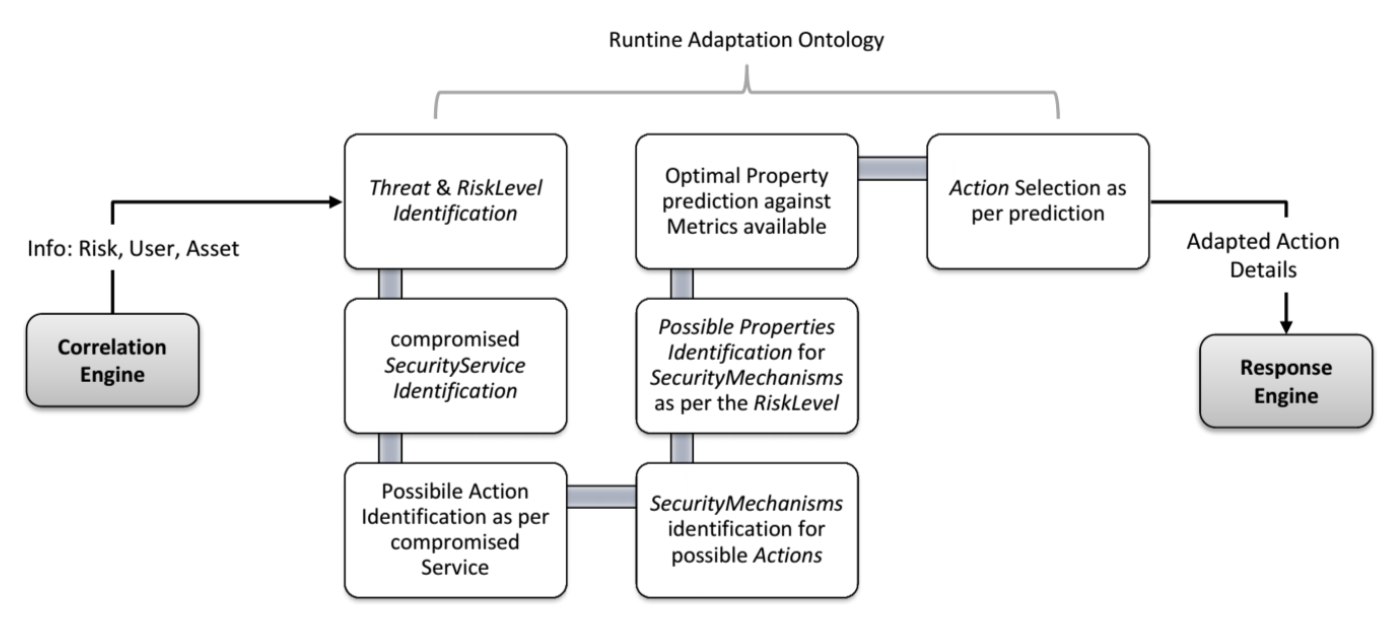
\includegraphics[width=0.7\textwidth]{imagens/edas-adaptation-process.png}
\caption{EDAS - processo de segurança adaptativa}
\label{edas-adaptation-process}
\end{figure}

Uma função de predição escolhe a ação de adaptação com o máximo de utilidade. Os pesos subjetivos são atribuídos a métricas afetadas para cada propriedade, os quais correspondem à utilidade geral da propriedade (para ser usada na ação adaptada) para um usuário específico. As métricas refletem parâmetros, como usabilidade, confiabilidade, custo do serviço, etc., que podem ser influenciados negativamente ou positivamente por uma propriedade de segurança selecionada. As métricas são agrupadas em três categorias, \textit{User}, QoS e \textit{Security}, para capturar influências sobre preferências de usuários, QoS e confiabilidade de segurança.

Os autores descrevem um cenário da IoT-eHealth no qual um paciente residindo em casa, está equipado com vários sensores corporais. Seus sinais vitais são monitorados através desses sensores e são transmitidos através de uma rede sem fio ou celular para um local remoto do hospital para posterior diagnóstico. O paciente freqüentemente usa seu \textit{smartphone}, parte dessa infraestrutura, instalado com um aplicativo de eHealth para acompanhar o estado de saúde, bem como para pagamentos de cobranças diversas além do uso pessoal. Com isto, um situação adversa é descrita onde um adversário com acesso ao  \textit{smartphone} tenta se autenticar no aplicativo de \textit{eHealth}. Desta forma, a EDAS deve levar em consideração os diferentes contextos para escolha da melhor opção de mitigação.
% No artigo não ocorre a prototipação e testes, mas na tese acredito que sim.

%%%%%%%%%%%%%%%%%%%%%%%%%%%%%%%%%%%%%%%%%%%%%%%%%%%%%%%%%%%%%%%%

\subsection{Managing Context Information for Adaptive Security in IoT environments} % 2015

Para abordar os desafios de modelagem e desenvolvimento de mecanismos de segurança cientes de contexto para a IoT, os autores deste trabalho definiram dois objetivos. Por um lado, o trabalho visa fornecer uma visão geral das implicações de segurança para os estágios do ciclo de vida do gerenciamento de contexto na IoT. Por outro lado, com base em um \textit{framework} de segurança para IoT proposto em \cite{bernabe14}, busca-se apresentar como as informações contextuais podem ser usadas por outros componentes deste \textit{framework} para capacitar objetos inteligentes com ciência de contexto ao tomar decisões de segurança \cite{ramos15}.


A Figura \ref{arm-framework} apresenta o \textit{framework} de segurança para IoT concebido em \cite{bernabe14}, no qual o grupo funcional de segurança é detalhado. Por um lado, o \textit{framework} amplia os componentes de segurança da \textit{Architecture Reference Model} (ARM) (ou seja, \textit{Authentication}, \textit{Authorization}, \textit{KEM}, \textit{Identity Management}, e \textit{Trust \&\& Reputation}) com a inclusão do \textit{Group Manager} e do \textit{Context Manager}. O primeiro pretende lidar com mecanismos de compartilhamento de dados mais flexíveis em que um grupo de objetos inteligentes podem ser envolvidos, enquanto a segurança e a privacidade são preservadas. O último é proposto para permitir a concepção de mecanismos de segurança cientes ao contexto para IoT, bem como para considerar as implicações de segurança durante as diferentes etapas do ciclo de vida do gerenciamento de contexto. Por outro lado, o \textit{framework} de segurança propõe as principais interações entre esses componentes de segurança, de modo a permitir a modelagem de mecanismos de segurança inovadores e adequados, a serem explorados em cenários da IoT.


\begin{figure}[ht]
\centering
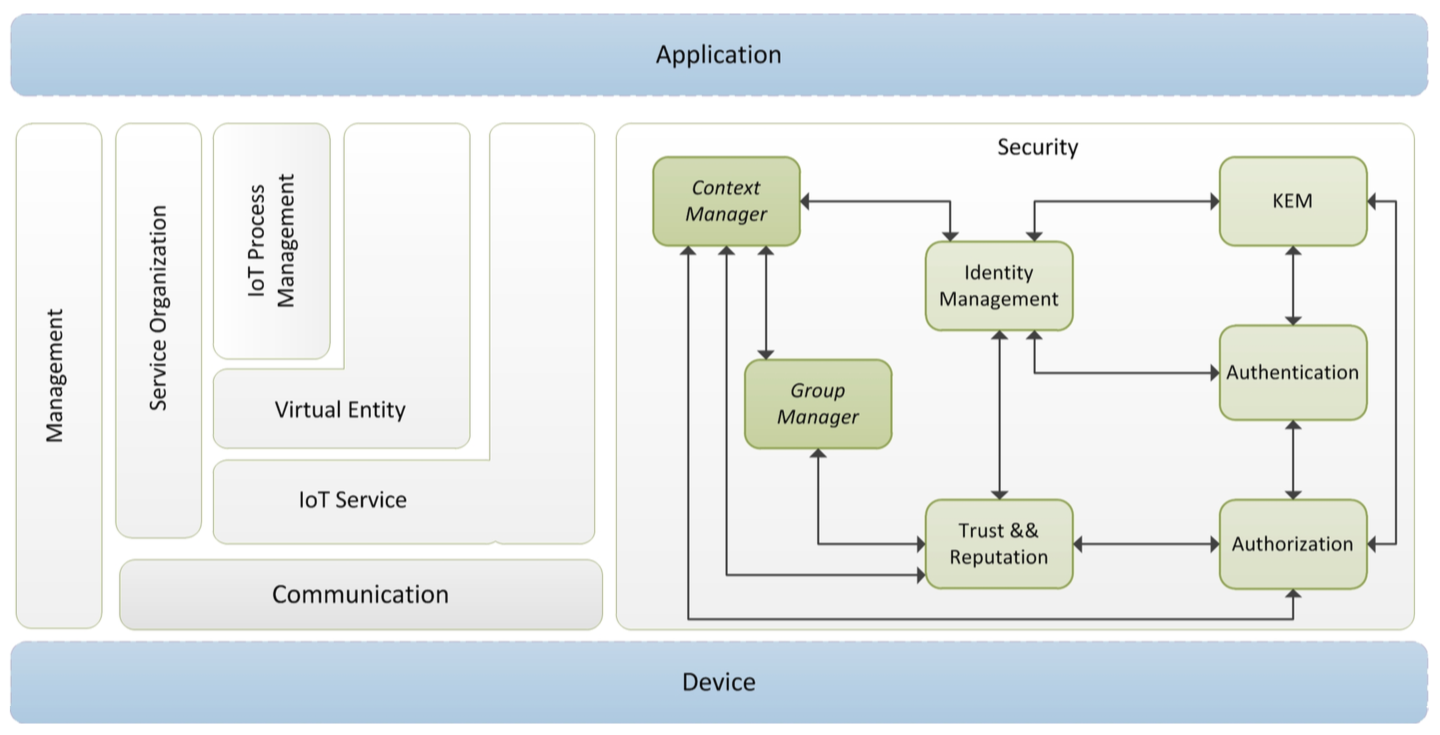
\includegraphics[width=0.7\textwidth]{imagens/arm-framework.png}
\caption{Framework de segurança ciente de contexto para IoT}
\label{arm-framework}
\end{figure}

Este trabalho tem como foco o Gerenciador de Contexto (\textit{Context Manager}), bem como as principais interações com outros componentes de segurança, a fim de tornar as decisões de segurança de objetos inteligentes cientes de contexto. Além disso, são propostos diferentes estágios para o ciclo de vida do gerenciamento de contexto, bem como um conjunto de diretrizes sobre implicações de segurança durante essas fases.

A Figura \ref{context-manager-overview} mostra os principais estágios considerados para o Gerenciador de Contexto do \textit{framework} de segurança. Essas etapas são extraídas das fases do ciclo de vida do contexto, que são propostas em \cite{perera14}. Antes de descrever essas etapas, deve-se destacar que o Gerenciador de Contexto pode ser instanciado de maneira diferente dependendo da entidade da IoT que está sendo considerada. Por exemplo, enquanto os \textit{smartphones} atuais podem ser capazes de implantar toda a funcionalidade das diferentes etapas, outros dispositivos da IoT com mais restrições de recursos, só poderiam implementar um subconjunto. No caso de sensores ou atuadores, eles podem implantar um subcomponente do comunicador de contexto, mas não a funcionalidade de raciocínio.
 
 \begin{figure}[ht]
\centering
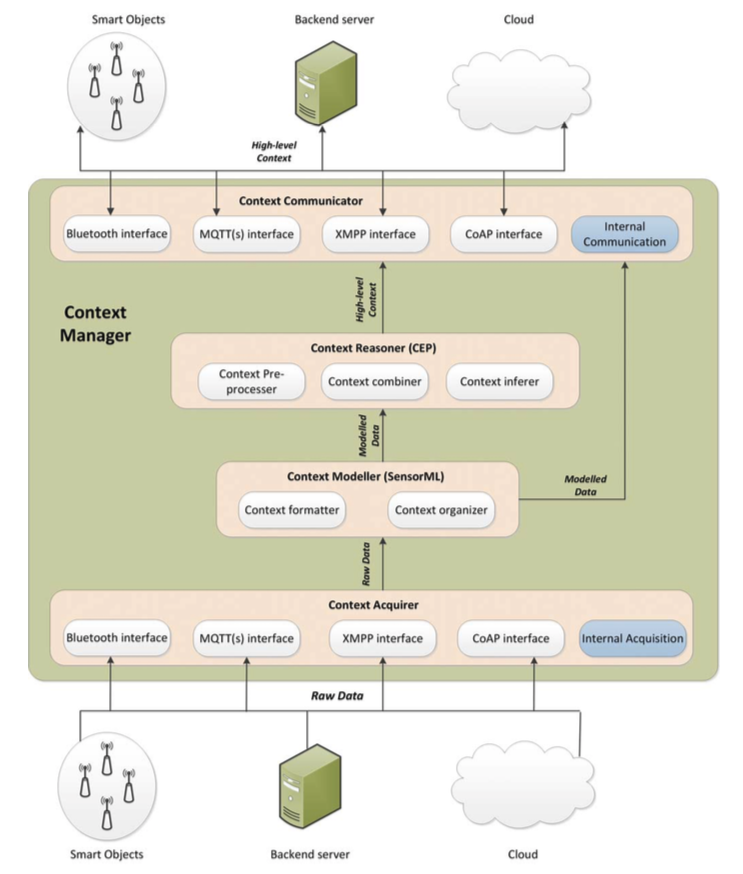
\includegraphics[width=0.7\textwidth]{imagens/context-manager-overview.png}
\caption{Visão geral do Gerenciador de Contexto}
\label{context-manager-overview}
\end{figure}


O Gerenciador de Contexto é dividido em quatro etapas principais. Em primeiro lugar, durante a fase de aquisição, o \textit{Context Acquirer} obtém informações de contexto a serem processadas. Esses dados podem ser provenientes de outras entidades internas (por exemplo, um acelerômetro no caso de um \textit{smartphone}) ou de outros objetos inteligentes no ambiente monitorado (por exemplo, um sensor de temperatura). Nesse caso, as informações de contexto podem ser adquiridas através de diferentes protocolos de comunicação empregados na IoT, como o \textit{Constrained Application Protocol} (CoAP), \textit{Extensible Messaging and Presence Protocol} (XMPP) ou \textit{Message Queue Telemetry Transport} (MQTT). Essas comunicações podem ser realizadas entre dispositivos com restrições de recursos, e precisam ser protegidas para que o Gerenciador de Contexto somente processe informações provenientes de objetos inteligentes legítimos. Enquanto alguns destes protocolos fornecem opções de segurança por meio de diferentes mecanismos (por exemplo, \textit{Datagram Transport Layer Security} (DTLS) no caso do CoAP), atualmente, a implementação de mecanismos de segurança para esses protocolos é um tópico de pesquisa. 
 
Depois que a informação contextual é adquirida, o conjunto de dados brutos é encaminhado para o componente \textit{Context Modeller} para serem interpretados e modelados de acordo com um modelo de contexto comum. Para esse fim, o subcomponente  \textit{Context formatter} é responsável por traduzir dados brutos para um formato comum que pode ser interpretado pelas camadas superiores do Gerenciador de Contexto. Para a modelagem das informações contextuais nos ambientes da IoT, é necessário considerar um balanço entre o grau de expressividade do modelo e a viabilidade a ser implantada em certos tipos de dispositivos. Portanto, para o Gerenciador de Contexto proposto, foi selecionado o \textit{Sensor Model Language} (SensorML) \cite{ocg18} (na versão \textit{JavaScript Object Notation} (JSON)) como uma alternativa flexível e gerenciável para a representação de informações contextuais em dispositivos da IoT. SensorML fornece modelagem de informações com base em pares chave-valor e e marcações, o que permite uma representação simples de dados de contexto. Desta forma, uma vez que a informação contextual é modelada, o subcomponente \textit{Context organizer} é responsável por validar o conjunto de dados modelados e adicioná-los ao repositório de informações contextuais do objeto inteligente.

Na próxima etapa, o \textit{Context Reasoner} é responsável por deduzir informações de contexto de alto nível sobre os dados modelados fornecidos pela etapa anterior. Para isso, são realizadas três tarefas principais. Em primeiro lugar, os dados modelados são enviados para o \textit{Context Pre-processer} que irá descartar dados ambíguos e imprecisos, ou provenientes de entidades não confiáveis e atribuir menor prioridade aos dados de contexto provenientes de objetos inteligentes com uma reputação questionável. 

Uma vez que os dados de contexto foram pré-pré-processados, a informação contextual é combinada pelo \textit{Context combiner} com dados de diferentes entidades levando em consideração a prioridade dos dados contextuais para criar uma visão de contexto mais completa. 

Finalmente, durante a fase de inferência, o conjunto de dados combinados é usado para produzir informações de contexto de alto nível através do \textit{Context inferer}. Este processo também pode estar ciente das preferências de segurança e privacidade do objeto inteligente. Existe uma ampla gama de técnicas de raciocínio de contexto que podem ser aplicadas, como por exemplo, regras, lógica difusa, ontologias ou lógica probabilística. Nesse sentido, dado o alto grau de dinamismo e ubiquidade da IoT, a tecnologia de Processamento de Eventos Complexos, do inglês \textit{Complex Event Processing} (CEP), fornece meios para processar eventos derivados de informações contextuais provenientes de diferentes entidades. Especificamente, fornece um procedimento apropriado para filtrar, agregar e mesclar dados de diferentes fontes em tempo de execução. A CEP é uma tecnologia bem conhecida baseada em regras, fácil de estender e de menor uso de recursos do que outras técnicas de raciocínio (por exemplo, ontologias), o que favorece sua adoção para o paradigma da IoT.

Durante a última etapa, informações contextuais de alto nível são enviadas para outras entidades (por exemplo, outros objetos inteligentes, servidores ou nuvem para processamento posterior), usando o \textit{Context Communicator}. Neste caso, as considerações de segurança do \textit{Context acquirer} também devem ser levadas em consideração por este componente para proteger as informações que estão sendo disseminadas. Além disso, a comunicação de informações contextuais de alto nível deve basear-se nas especificações NGSI-9 e NGSI-10 \cite{oma12}, permitindo uma interface comum para troca de dados de contexto com outras entidades. Outras considerações de segurança podem ser levadas em consideração quanto à freqüência ou granularidade desses dados, pois isso pode prejudicar a privacidade do objeto inteligente (ou do proprietário). Além das interfaces de comunicação externas, o comunicador de contexto mantém uma interface de comunicação interna para enviar informações de contexto de alto nível para outros componentes do \textit{framework} de segurança. Essas interações destinam-se a criar uma visão de segurança adaptativa para o paradigma da IoT.

Após a descrição dos componentes do Gerenciador de Contexto, conforme observa-se na Figura \ref{context-aware-adaptive-security}, os autores apresentam as principais interações projetadas entre o gerenciador e outros componentes de segurança para gerar as decisões de segurança sobre os objetos inteligentes promovendo a segurança adaptativa. 

 \begin{figure}[ht]
\centering
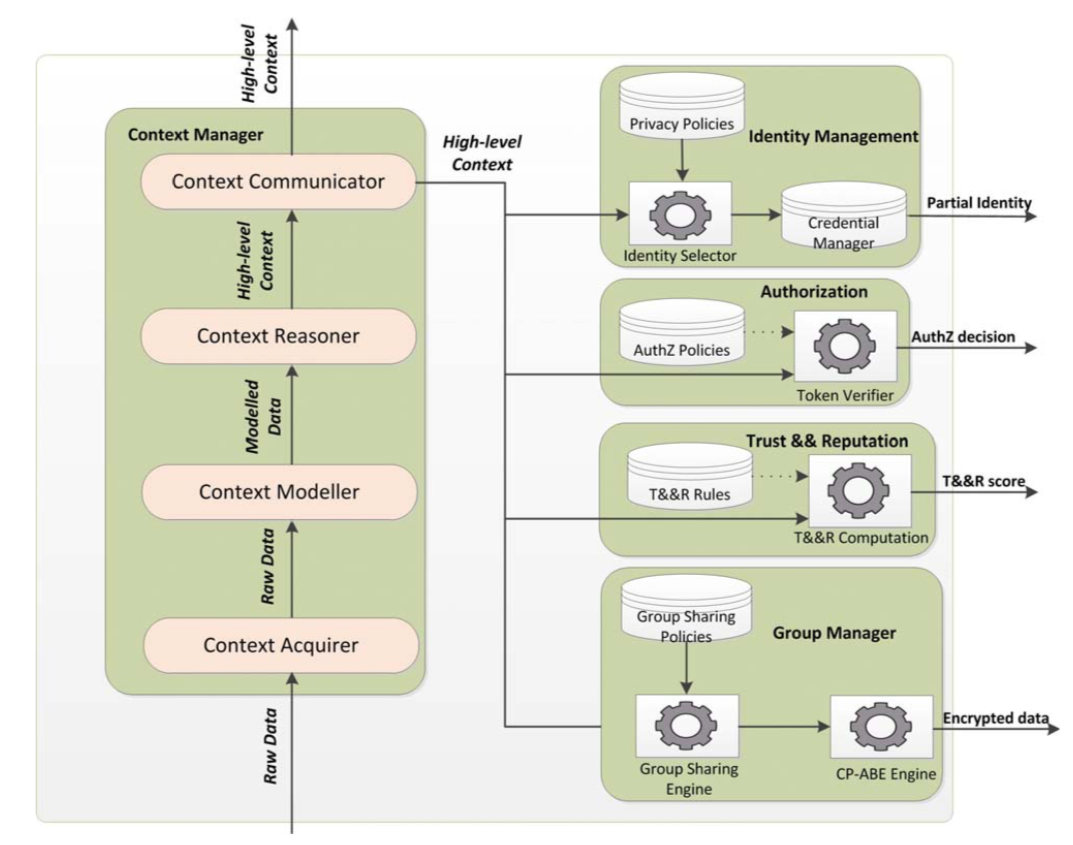
\includegraphics[width=0.7\textwidth]{imagens/context-aware-adaptive-security.png}
\caption{Interações do \textit{framework} para mecanismos de segurança adaptativa cientes de contexto}
\label{context-aware-adaptive-security}
\end{figure}

O componente \textit{Identity Management} (IdM) é responsável por gerenciar as identidades de um objeto inteligente de forma a preservar a privacidade. O \textit{Authorization} é baseado em uma combinação de modelos e técnicas de controle de acesso sendo implantado para gerar tokens de autorização. O componente \textit{Trust \&\& Reputation} permite estabelecer um ambiente de IoT seguro e confiável, onde os usuários podem interagir com os serviços da IoT com segurança. Enquanto o \textit{Group Manager} baseia-se no uso do esquema de criptografia \textit{Ciphertext Policy Attribute Based Encryption} (CP-ABE) para permitir um mecanismo seguro de compartilhamento de dados com grupos de objetos inteligentes.
 
%%%%%%%%%%%%%%%%%%%%%%%%%%%%%%%%%%%%%%%%%%%%%%%%%%%%%%%%%%%%%%%%

\subsection{An Ontology-based Security framework for Decision-making in Industrial Systems} % 2016

Este trabalho propõe uma arquitetura para \textit{framework} de segurança adaptativa (vide Figura \ref{iotsec-architecture}) baseada no modelo MAPEK utilizando uma ontologia para a tomada de decisões visando melhorar a segurança da informação em sistemas industriais \cite{mozzaquatro16}. A ontologia IoTSec \cite{mozzaquatro15} empregada na base de conhecimento contribui para sustentar o sistema usando consultas de informações contextuais coletadas no ambiente. A principal contribuição desta abordagem é validada como uma integração com o projeto \textit{Cloud Collaborative Manufacturing Networks} (C2NET\footnote{http://c2net-project.eu/}) para garantir propriedades de segurança em alguns cenários críticos.

\begin{figure}[ht]
\centering
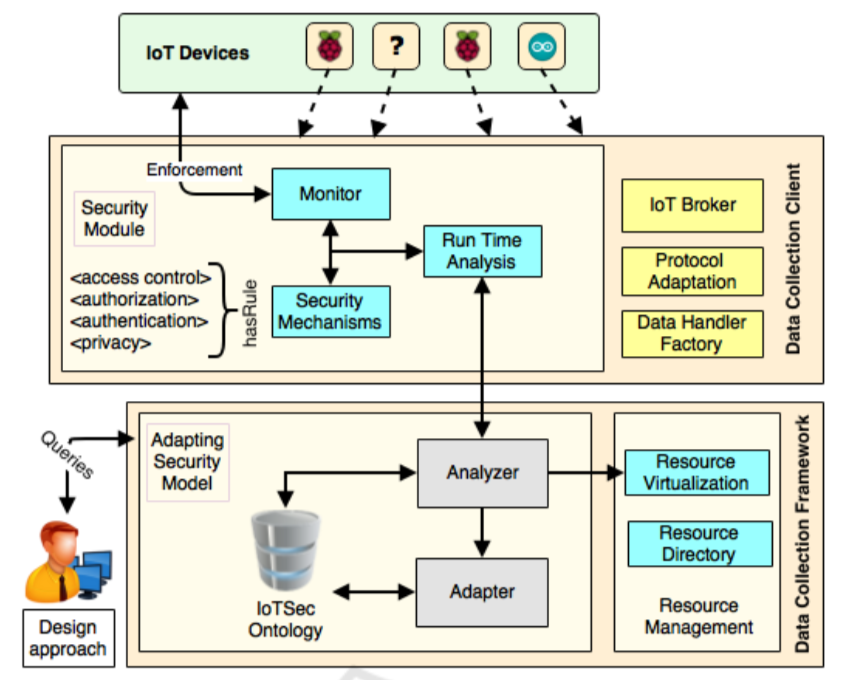
\includegraphics[width=0.7\textwidth]{imagens/iotsec-architecture.png}
\caption{Uma arquitetura para \textit{framework} de segurança adaptativa baseada em ontologia integrada com a plataforma C2NET.}
\label{iotsec-architecture}
\end{figure}

A IoTSec, aprensetada na Figura \ref{iotsec-ontology}, é uma ontologia de referência para a segurança na IoT proposta em \cite{mozzaquatro15} para explorar aspectos das relações entre os componentes básicos da análise de risco da ISO/IEC 13335-1:2004 e da \textit{National Institute of Standards and Technology} (NIST) \textit{Special Publication} 800-12, como: \textit{Assets}, \textit{Threats}, \textit{SecurityMechanism}, \textit{Vulnerability} and \textit{Risk}. A Figura \ref{iotsec-ontology} apresenta um arranjo de classes de alto nível para modelar a IoTSec.

\begin{figure}[ht]
\centering
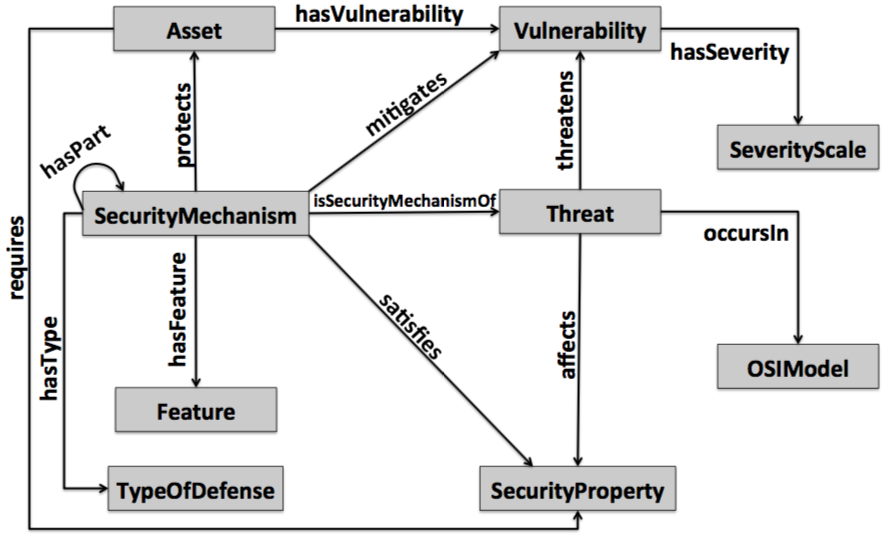
\includegraphics[width=0.7\textwidth]{imagens/iotsec-ontology.png}
\caption{Ontologia de referência para segurança na IoT \cite{mozzaquatro15}}
\label{iotsec-ontology}
\end{figure}

A plataforma colaborativa C2NET tem como base a computação na nuvem permitindo que pequenas e médias empresas otimizem os seus recursos logísticos e de produção com base em dinâmicas colaborativas de procura, produção ou expedição. Um dos principais problemas das cadeias de abastecimento tradicionais está relacionado à centralização das abordagens de tomada de decisão, o que dificulta a reação das empresas considerando a dinamicidade dos mercados atuais. De acordo com isso, a plataforma C2NET é proposta para contribuir em vários aspectos da fabricação industrial, explorando a coleta de dados de dispositivos da IoT presentes nas empresas. No entanto, esses dispositivos são vulneráveis a várias ameaças e precisam ser abordados usando mecanismos de segurança. Além disso, alguns desses dispositivos usam diferentes tecnologias da IoT e a plataforma C2NET explora a interoperabilidade baseada em tecnologias da web semântica.

O \textit{framework} de segurança é proposto com duas abordagens para melhorar os problemas de segurança da plataforma C2NET: modelagem e tempo de execução. A abordagem de modelagem explora os conhecimentos anteriores para adoção de novas tecnologias ou produtos considerando questões de segurança. Esta opção impacta nas empresas, pois o responsável pelas compras geralmente não possui experiência em segurança da informação e a compra de produtos é realizada sem análise de segurança.

%On the other hand, run time approach monitors IoT devices based on security metrics and attributes to identify malicious behaviors in the smart environ- ment. Consequently, configurations and/or rules need to be adapted according the knowledge base, when alerts are triggered by security tools. For that, IoT ontology contributes to identify relations between threat, asset, vulnerability, security mechanism and security property. Nevertheless, the adapter infers in new information on knowledge base to deploy new approaches for specifics situations or malicious behaviors.
% [ric] está estranho este paragrafo, tentar entender lendo o texto
Por outro lado, a abordagem em tempo de execução monitora os dispositivos da IoT com base em métricas e atributos de segurança para identificar comportamentos maliciosos no ambiente. Conseqüentemente, as configurações e/ou regras precisam ser adaptadas de acordo com a base de conhecimento, quando os alertas são acionados por ferramentas de segurança. Para isso, a ontologia contribui para identificar as relações entre ameaça, ativos, vulnerabilidades, mecanismos de segurança e propriedades de segurança. No entanto, o adaptador infere novas informações sobre a base de conhecimento para implantar novas abordagens para situações específicas ou comportamentos maliciosos.

Para validação da proposta dois cenários foram desenvolvidos sobre o setor metalúrgico buscando aplicar a estrutura de segurança baseada em ontologia para melhorar os problemas de segurança entre os dispositivos da IoT e a plataforma C2NET. Os autores observam que o trabalho considera que os cenários são vulneráveis apenas à ameaças digitais, como divulgação de informações, ataques de repetição, \textit{spoofing} e outros ataques a dispositivos inteligentes.

%%%%%%%%%%%%%%%%%%%%%%%%%%%%%%%%%%%%%%%%%%%%%%%%%%%%%%%%%%%%%%%%
\subsection{Efficient Security Adaptation framework for Internet of Things} % 2016

Neste artigo os autores destacam que de acordo com Shnitko (2004)\nocite{shnitko04}, os problemas principais e típicos da segurança em sistemas complexos são: o uso ineficiente e inadequado de métodos e ferramentas de segurança disponíveis e a dispersão de recursos ao tentar resolver diversos problemas de segurança ao mesmo tempo. Com isso, eles assumem que esses problemas precisam de soluções eficientes, o que leva à demanda por métodos de segurança adaptativos. Desta forma, o artigo apresenta um \textit{framework} genérico denominado \textit{Security Adaptation Reference Monitor} (SARM) como uma proposta para solução destes problemas, visto que ele emprega o paradigma autonômico e é desenvolvido especialmente para ambientes suportados por redes sem fio altamente dinâmicas \cite{elmaliki16}.

O SARM realiza os ajustes dos parâmetros de segurança levando em consideração o risco do ambiente atual e o desempenho do sistema, especialmente no que se refere à otimização do seu consumo de energia. Isto ocorre sob as políticas e as restrições de intervenção em tempo de execução dos usuários. Assim, de acordo com os autores, o \textit{framework} se difere dos outros por:

\begin{itemize}
\item utilizar um sistema de controle de feedback de segurança autônoma;
\item empregar mecanismos de segurança dinâmicos e em evolução relacionados ao monitoramento de contextos;
\item realizar o gerenciamento de energia explícita;
\item lidar com a mobilidade dos atacantes.
\end{itemize}

O foco principal deste trabalho é a adaptação de segurança em ambientes de comunicação móvel e sem fio. Além disso, de acordo com autores, a melhor maneira de implementar o \textit{framework} para cada programa de comunicação seria integrá-lo no \textit{kernel} e, consequentemente, ter o controle geral da segurança do ambiente. Assim, todos os programas de comunicação teriam que interagir com o SARM para obter acesso aos recursos de comunicação.

O SARM foi proposto como um \textit{framework} genérico pois os autores consideram que implementar e escolher um sistema de segurança adaptativa depende de alguns fatores que estão correlacionados, como: o custo de aquisição; custo de manutenção; usabilidade, e; eficiência. Com isto, a proposta foi concebida seguindo uma metodologia de construção modular de blocos de modo a facilitar a integração e ocultar a complexidade interna do sistema. Além disso, essa abordagem permite uma expansão gradual para atender aos novos requisitos da IoT devido sua constante evolução. Para reagir em tempo real a qualquer ameaça, o SARM baseia-se em informação de feedback buscando reduzir a intervenção humana.

Três componentes principais do sistema autônomo, disposto na Figura \ref{sarm-description} foram identificados no projeto: o primeiro é uma unidade funcional, o qual desempenha funções operacionais, sendo responsável por selecionar parâmetros de segurança adequados, como acesso eficiente à rede; o segundo é uma unidade de gerenciamento, que controla a unidade funcional; e o componente final consiste em entradas e saídas. Os parâmetros de segurança são definidos como qualquer algoritmo ou mecanismo que possa aprimorar a segurança, mas que também tenha a capacidade de não tomar medidas de segurança, a menos que seja realmente necessário. Isto inclui a escolha do acesso adequado à rede, uma vez que algumas tecnologias de comunicação de rede são mais seguras, porém com maiores níveis de consumo de energia, enquanto outras são menos seguras, e consequentemente possuem menores níveis de consumo de energia.

\begin{figure}[ht]
\centering
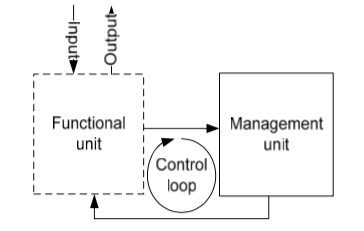
\includegraphics[width=0.7\textwidth]{imagens/sarm-description.png}
\caption{SARM - descrição do sistema autônomo}
\label{sarm-description}
\end{figure}


Os componentes mencionados foram estendidos com base na arquitetura de segurança adaptativa. Desta forma, o \textit{framework} foi descrito como uma quintupla: AS = (A,X,Q,Up,Uf). A é composto por componentes do sistema e um conjunto de propriedades. Esses componentes pertencem a informações relacionadas ou não (como QoS, por exemplo) à segurança.  O contexto X refere-se à circunstância de qualquer interação entre um usuário e o sistema. As dimensões de adaptividade Q são relacionadas à QoS ou segurança, e fornecem uma visão de alto nível dos usuários do sistema. As preferências do usuário, representadas pela sigla Up, expressam restrições e requisitos dos usuários. A função de utilidade (Uf) expressa a qualidade da adaptação para um usuário ou rede.

Após definir explicitamente os elementos de um sistema adaptativo, os autores realizam o mapeamento dos mesmos em um sistema autônomo, conforme observa-se na Figura \ref{sarm-framework}. Para a unidade funcional, foram adicionadas as preferências de usuários e os parâmetros de segurança. Depois disso, foi adicionado um elemento sensorial para levar em consideração o contexto. Para a unidade de gerenciamento, fora definidas as políticas e logs para segurança de curto e longo prazo  ou para análises de segurança e monitoramento de QoS.  Os blocos de risco, vulnerabilidades e desempenho foram baseados no módulo de gerenciamento de risco.

\begin{figure}[ht]
\centering
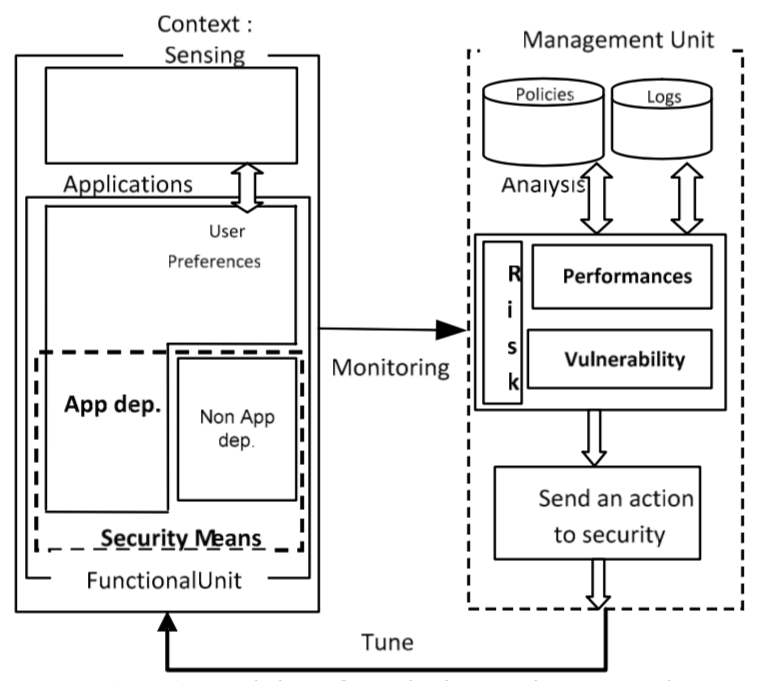
\includegraphics[width=0.7\textwidth]{imagens/sarm-framework.png}
\caption{SARM - fundamentos do \textit{framework} genérico para segurança adaptativa}
\label{sarm-framework}
\end{figure}

Os parâmetros de segurança são definidos como qualquer algoritmo ou mecanismo que possa aprimorar a segurança, mas que também tenha a capacidade de não tomar medidas de segurança, a menos que seja realmente necessário. Também inclui a escolha do acesso adequado à rede, uma vez que algumas tecnologias de comunicação de rede são mais seguras, com maiores níveis de consumo de energia, enquanto outras são menos seguras, com menores níveis de consumo de energia.

% [ric] Acho que posso detalhar mais aqui, sem entrar em detalhes mas descrevendo um pouco o cenário
Os detalhes de implementação e experimentação do SARM junto à uma série de simulações e avaliações incluindo as métricas de avaliação, especialmente referentes ao consumo de energia, são expostas em \cite{elmaliki14}.

%%%%%%%%%%%%%%%%%%%%%%%%%%%%%%%%%%%%%%%%%%%%%%%%%%%%%%%%%%%%%%%%

\section{Discussão dos Trabalhos Relacionados}

Conforme destacado na introdução deste trabalho, de acordo com a literatura (em especial alguns ``\textit{surveys}''), inclusive com os trabalhos identificados no estado da arte, os seguintes aspectos foram identificados como problemas relacionados as pesquisas em arquiteturas/modelos de segurança adaptativa:

\begin{enumerate}
\item  se concentram em apenas um serviço/objetivo de segurança, como a autenticação \cite{aman14}, \cite{elkhodary07};
\item as abordagens existentes não definem todo o ciclo de adaptação MAPE \cite{yuan12}.
\item fornecem uma arquitetura genérica sem detalhar os métodos usados em cada componente  \cite{aman14}, \cite{yuan12};
\item a falta de detalhes nas arquiteturas genéricas dificulta a reutilização e extensibilidade das abordagens propostas \cite{yuan12};
\end{enumerate}

No que diz respeito ao primeiro e segundo problemas elencados, o mapeamento sistemático buscou filtrar esta questão, sendo selecionados apenas artigos onde as arquiteturas/modelos concebidos podem ser aplicados em diferentes objetivos de segurança e que contemplam o ciclo MAPE por inteiro. Já quanto ao terceiro e quarto tópicos levantados, é possível observar que o primeiro trabalho apresentado neste capítulo \cite{habtamu12} - o qual é concebido por uma das referências na área (Abie Habtamu) - possui tal limitação, a qual é tratada apenas em alguns dos demais trabalhos.

Tendo estas observações em vista, a tabela \ref{comparacao-estado-da-arte} busca apresentar algumas das características consideradas para comparação entre os trabalhados identificados como estado da arte em segurança adaptativa para IoT. O sinal de hífen (``-'') na tabela representa a falta de informações ou limitação por parte do trabalho quanto a referida característica. A seguir é apresentada uma breve descrição das características selecionadas:

\begin{itemize}
\item coleta: uma dos desafios na IoT diz respeito a coleta de eventos de dispositivos com recursos limitados, logo, esta característica busca identificar se são destacados no trabalho os detalhes para coleta dos eventos;
\item normalização: uma vez que o foco é na IoT, a heterogeneidade e a consequente diversidade no formato dos eventos produzidos deve ser tratada, sendo assim, este tópico identifica se a proposta detalha a estratégia utilizada para normalização;
\item correlação: estratégia utilizada para correlação dos diferentes contextos identificados para identificação de situações de interesse;
\item armazenamento: determina a tecnologia de armazenamento do conhecimento empregada, sendo relevante por fatores de expressividade, escalabilidade e usabilidade;
\item implementação: visa caracterizar o nível de detalhamento do protótipo desenvolvido para validação do trabalho, podendo ser 
``Não'', ``Parcial'' e ``Sim'';
\item extensibilidade: representa a possibilidade de extensão da arquitetura/modelo proposto;
\item reusabilidade: busca evidenciar se o trabalho descreve detalhes suficientes que permitem o reuso da proposta, sendo passível de replicação dos testes realizados;
\item maturidade: descreve o nível de maturidade da abordagem em função da validação desenvolvida e da comunidade em torno das tecnologias empregadas;
\item cenário: caracteriza a área de estudo do cenário de avaliação;
\item escalabilidade: procura identificar limitações ou competências quanto a escalabilidade da proposta uma vez que na IoT o volume de dados tratados em função da quantidade de dispositivos adquirindo contextos é um desafio a ser considerado.
\end{itemize}

\begin{table}[ht]
\centering
\caption{Tabela comparativa entre os trabalhos identificados como estado da arte em segurança adaptativa}
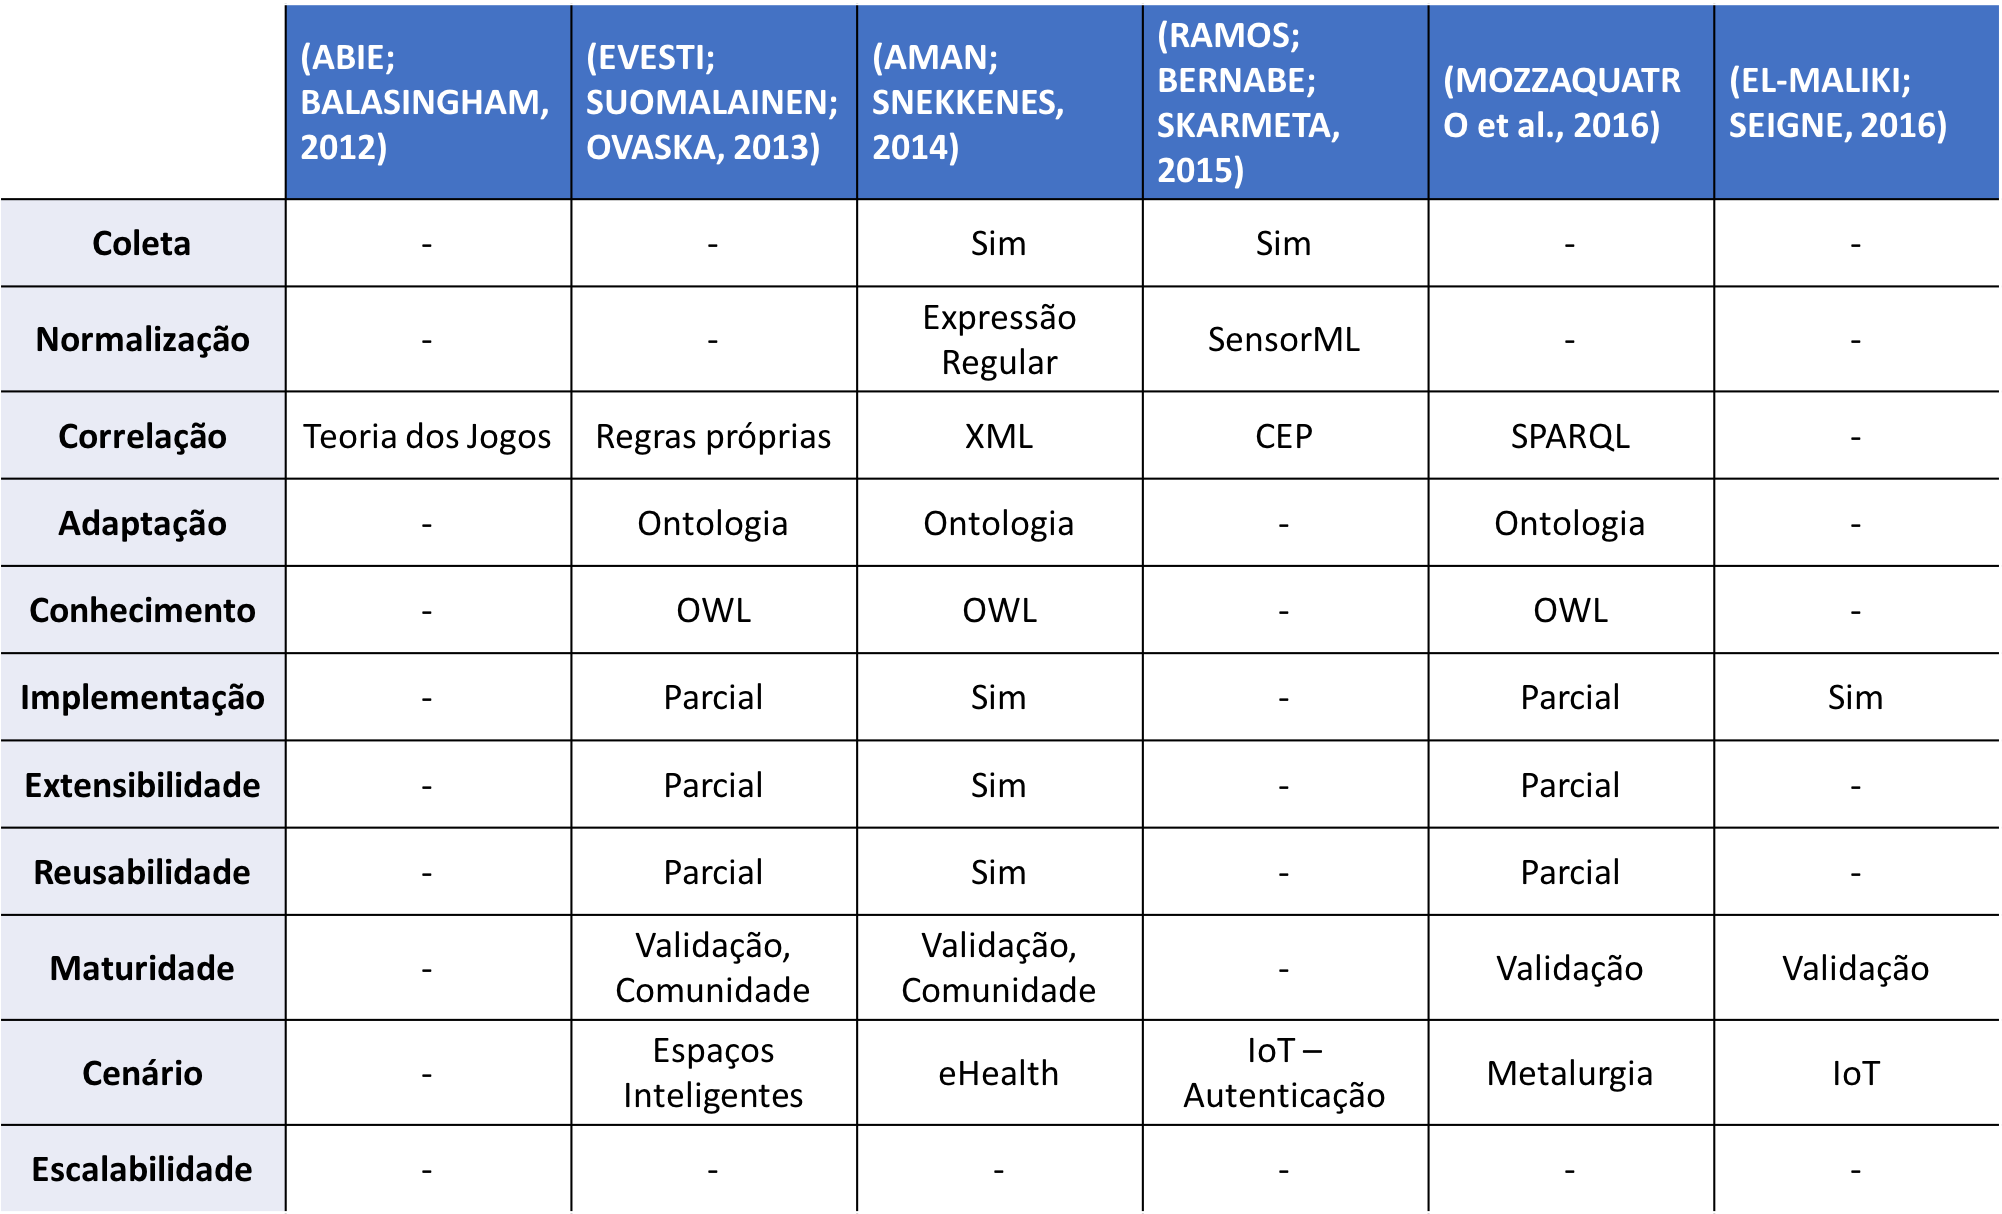
\includegraphics[width=1.0\textwidth]{imagens/comparacao-estado-da-arte.png}
\label{comparacao-estado-da-arte}
\end{table}

Em \cite{evesti13c}, exceto no que tange o emprego da ontologia, os detalhes de implementação identificados por este autor são considerados superficiais e as tecnologias adotadas (como por exemplo, Qt C++) são fortemente dependentes da plataforma empregada. Também não são descritos de forma clara as tecnologias envolvidas para coleta e normalização de eventos. Com isso, apesar do autor Antti Evesti ressaltar a sua abordagem como extensível e reutilizável, para o autor deste trabalho, esta afirmação pode ser aplicada apenas no que tange a ontologia, porém não no seu trabalho de maneira geral.

De forma geral, o quesito maturidade, a maior parte dos trabalhos apresentou cenários para validação da proposta, porém, as tecnologias envolvidas possuem restrição quanto à sua adoção pela comunidade, em especial pela utilização de ontologias, que apesar de ser um tópico importante de pesquisa em desafios de segurança da informação, não é possível afirmar que a sua adoção vem sendo praticada na área.

Percebe-se também que a adoção de ontologias por parte dos trabalhos \cite{evesti13c}, \cite{aman14} e \cite{mozzaquatro16} implica em dificuldades de escalabilidade, sendo em geral uma problemática levantada como limitações em seus trabalhos ou teses derivadas. Além disso, em \cite{aman14}, a tecnologia OSSIM empregada é reconhecida por possuir problemas de estabilidade e escalabilidade \cite{gartner15}, \cite{infosecnirvana14}.

O trabalho \cite{ramos15}, por sua vez, apresenta um modelo genérico, sem detalhar os modelos e tecnologias empregadas. Assim assim, ele destaca alguns dos protocolos geralmente envolvidos para coleta de eventos na IoT, como o \textit{Constrained Application Protocol} (CoAP), \textit{Extensible Messaging and Presence Protocol} (XMPP) ou \textit{Message Queue Telemetry Transport} (MQTT).

El-Maliki apresenta em sua tese \cite{elmaliki14} uma série de testes e simulações realizadas para validação, avaliando em especial a latência decorrente do uso da criptografia e o consumo de energia, os quais evidenciam estratégias de implementação em diferentes cenários da IoT. Apesar disso, o protótipo é fortemente associado ao estudo de caso, não sendo uma abordagem voltada para eventos, consequentemente não possuindo detalhes sobre a coleta de eventos, sua normalização, correlação, armazenamento, bem como estratégia empregada na adaptação. Além disso, não é uma característica a possibilidade de extensão e reuso da proposta.

\section{Considerações do Capítulo}

Este capítulo apresentou os trabalhos identificados como estado da arte em arquiteturas ou \textit{frameworks} genéricos de segurança adaptativa para IoT. O processo para esta análise seguiu o mapeamento sistemático da literatura. Os trabalhos foram descritos em termos do modelo proposto, buscando detalhar as estratégias de concepção e prototipação. Finalmente, foi realizada uma comparação entre os mesmos seguindo características consideradas oportunas considerando as críticas e desafios identificados durante esta revisão. 

%%%%%%%%%%%%%%%%%%%%%%%%%%%%%%%%%%%%%%%%%%%%%%%%%%%%%%%%%%%%%%%%%%%%%%%

\chapter{Considerações Finais}

O presente trabalho buscou apresentar uma revisão conceitual sobre segurança adaptativa para IoT. No decorrer da revisão foi possível perceber os diferentes desafios existentes na IoT que potencializam a segurança da informação enquanto estratégia para viabilização dos inúmeros benefícios decorrentes deste paradigma. 

Com isso, foi encaminhada a necessidade de arquiteturas para segurança adaptativa que promovam a adaptação dinâmica dos mecanismos de segurança de forma que as mudanças aplicadas não prejudiquem a eficiência, flexibilidade, confiabilidade e segurança dos ambientes da IoT. Tendo em vista a natureza ubíqua,
%\AY{ubíqua  - padronizar: ou pervasiva ou ubíqua} - feito
distribuída e dinâmica da IoT, as informações contextuais devem ser um dos principais componentes para conduzir o comportamento dos dispositivos a fim de tornar as decisões de segurança adequadas ao ambiente. 

Para a concepção dessas arquiteturas foi apresentado o ciclo de \textit{feedback} MAPE-K, o qual consiste de um método formal que estabelece as etapas a serem executadas para a adaptação. É importante salientar que para implementar cada umas destas etapas algumas questões devem ser respondidas. Além disso, um sistema adaptativo deve contemplar auto-atributos como: autoconfiguração, auto-otimização, autocura e autoproteção. Não obstante, pesquisas vem sendo desenvolvidas nessa área indicando a ciência de contexto como outro atributo a ser explorado.

Desta forma, a segurança adaptativa baseada em contexto envolve a coleta de informações contextuais tanto do sistema como do meio ambiente, medindo o nível de segurança e as métricas, realizando o processamento dessas informações coletadas e respondendo às mudanças (i) ajustando parâmetros internos, como esquemas de criptografia, protocolos de segurança, políticas de segurança, algoritmos, diferentes mecanismos de autenticação e autorização, alterando a QoS e automatizando a reconfiguração dos mecanismos de proteção e/ou (ii) fazendo mudanças dinâmicas na estrutura do sistema de segurança \cite{habtamu12}.

Atualmente, existem várias abordagens para segurança adaptativa \cite{elkhodary07, yuan12}. No entanto, conforme ressaltado no capítulo sobre o estado da arte, as abordagens existentes se concentram em objetivos de segurança específicos. Percebe-se também a falta no tratamento total do ciclo de \textit{feedback}, ou seja, as abordagens não definem todo o ciclo MAPE. Além disso, Yuan et al. observa que as arquiteturas genéricas não detalham os métodos usados em cada componente, o que dificulta a reutilização e extensibilidade das abordagens propostas. Com o mapeamento sistemático realizado neste trabalho, foi possível identificar que apesar dos avanços nas pesquisas em segurança adaptativa em diferentes frentes, os desafios mencionados continuam em aberto, existindo ainda poucas abordagens genéricas que detalhem a sua concepção, prototipação e estratégias de avaliação.

%\section{Perspectiva de Investigação}

%\section{Trabalhos Futuros}

%%%%%%%%%%%%%%%%%%%%%%%%%%%%%%%%%%%%%%%%%%%%%%%%%%%%%%%%%%%%%%%%%%%%%%%
\bibliography{bibliografia}
\bibliographystyle{abnt}

\end{document}